\listfiles
\documentclass{elsarticle}
%\documentclass[final,5p,times,twocolumn]{elsarticle}
\usepackage{hyperref}
\pdfstringdefDisableCommands{%
  \def\corref#1{}%
}
\usepackage{tabularx}
\usepackage{adjustbox}
\usepackage{afterpage}
\usepackage{algorithm,algorithmic}
\usepackage{amsfonts}
\usepackage{amsmath,amssymb}
\usepackage{booktabs}
\usepackage{color,colortbl}
\usepackage{comment}
\usepackage{float}
\usepackage{graphicx}
\usepackage{subcaption}
\usepackage{mathrsfs}
\usepackage{multirow}
\usepackage{pdflscape}
\usepackage{lineno,hyperref}
\usepackage{longtable}
\usepackage{siunitx}
\usepackage{tikz}
\usepackage{svg}
\usepackage{ulem}
\usepackage{booktabs}
\usepackage{multirow}

\modulolinenumbers[5]

\newcommand{\No}[1]{{\color{red}\sout{#1}}}
\newcommand{\Si}[1]{{\color{blue}#1}}

\usepackage{pgfplots}
\pgfplotsset{compat=1.9}
\usepgfplotslibrary{external}
\tikzexternalize

\newcommand{\diff}{\textit{diff}}
\newcommand{\gris}[1]{\textcolor{lightgray}{#1}}

\journal{Journal's name}

%%%%%%%%%%%%%%%%%%%%%%%
%% Elsevier bibliography styles
%%%%%%%%%%%%%%%%%%%%%%%
%% To change the style, put a % in front of the second line of the current style and
%% remove the % from the second line of the style you would like to use.
%%%%%%%%%%%%%%%%%%%%%%%

%% Numbered
%\bibliographystyle{model1-num-names}

%% Numbered without titles
%\bibliographystyle{model1a-num-names}

%% Harvard
%\bibliographystyle{model2-names.bst}\biboptions{authoryear}

%% Vancouver numbered
%\usepackage{numcompress}\bibliographystyle{model3-num-names}

%% Vancouver name/year
%\usepackage{numcompress}\bibliographystyle{model4-names}\biboptions{authoryear}

%% APA style
%\bibliographystyle{model5-names}\biboptions{authoryear}

%% AMA style
%\usepackage{numcompress}\bibliographystyle{model6-num-names}

%% `Elsevier LaTeX' style
%\bibliographystyle{elsarticle-num}
%%%%%%%%%%%%%%%%%%%%%%%

\begin{document}

\begin{frontmatter}

\title{Enhancing brain image segmentation: A metaheuristic approach to multi--threshold optimization}

%\tnotetext[mytitlenote]{Fully documented templates are available in the elsarticle package on % %\href{http://www.ctan.org/tex-archive/macros/latex/contrib/elsarticle}{CTAN}.
%}

%% or include affiliations in footnotes:
%\author[mymainaddress,mysecondaryaddress]{Elsevier Inc}
%\ead[url]{www.elsevier.com}

%\author[mysecondaryaddress]{Global Customer Service\corref{mycorrespondingauthor}}
%\cortext[mycorrespondingauthor]{Corresponding author}
%\ead{support@elsevier.com}

%\address[mymainaddress]{1600 John F Kennedy Boulevard, Philadelphia}
%\address[mysecondaryaddress]{360 Park Avenue South, New York}

\author{Fernando Ram\'irez$^{a}$}
\ead{fernando.ramirezs@postgrado.uv.cl}

\author{Emilio Flores$^{a}$}
\ead{emilio.flores@postgrado.uv.cl}

\author{Rodrigo Olivares\corref{cor}$^{a,}$}
\cortext[cor]{Corresponding author}
\ead{rodrigo.olivares@uv.cl}

\address{$^{a}$Escuela de Ingenier\'ia Inform\'atica, Universidad de Valpara\'iso, 2362905, Valpara\'iso, Chile.}

\begin{abstract}

Brain segmentation is vital for the accurate diagnosis and treatment of neurological disorders, given the complexity and vulnerability of the brain to various pathologies such as strokes and tumors. The challenge lies in achieving precise delineation of anatomical and pathological structures within medical images, particularly under varying conditions of image quality and tissue irregularities. To address this, we applied eight metaheuristic optimization algorithms---Reptile Search Algorithm, Orca Predator Algorithm, Bald Eagle Search, Grey Wolf Optimizer, Honey Badger Algorithm, Crow Search Algorithm, Harris Hawk Optimization, and Tuna Swarm Optimization---to improve the accuracy of multi-threshold segmentation methods like Kapur’s entropy, Tsallis entropy, and the Otsu method. The results reveal that the Grey Wolf Optimizer and Tuna Swarm Optimization stand out, with the Grey Wolf Optimizer demonstrating superior performance across key metrics such as Peak Signal to Noise Ratio and Structural Similarity Index. These outcomes highlight the potential of the Grey Wolf Optimizer for advanced brain tissue segmentation, offering significant advantages in clinical and research environments where precision is essential for effective medical intervention.

\end{abstract}

\begin{keyword}
Bio-inspired optimization algorithm \sep
Kapur's Entropy \sep
Tsallis Entropy \sep 
Otsu Method \sep 
Medical Image Segmentation.
\end{keyword}

\end{frontmatter}

\section{Introduction}

The brain, a crucial organ in the human body, not only coordinates vital functions and processes sensory and cognitive information, but it is also fundamental in the regulation of emotion, behavior, and overall bodily homeostasis~\cite{Raichle2010}. This makes the brain particularly important, but also highly vulnerable to various diseases such as strokes, tumors, and other neurological pathologies that can severely compromise both its structure and function~\cite{Fornito2015,Kreisl2008}. Evaluating these conditions often requires the use of advanced medical imaging techniques, such as magnetic resonance imaging (MRI), which provide detailed and high-resolution images of brain tissue, enabling clinicians to detect abnormalities that might otherwise go unnoticed~\cite{Young2007,Mehrabian2019}.

Over the years, image segmentation has seen significant evolution, transitioning from manual, labor-intensive methods to sophisticated automated techniques, in a field where medical professionals, including radiologists and neurologists, rely on precise and efficient diagnostic tools to ensure that the images they analyze lead to accurate diagnoses and effective treatment plans~\cite{Halder2019}. Researchers and scientists are continually striving to innovate by developing more advanced segmentation methods, improving both the accuracy and reliability of these tools. Traditionally, tools such as ImageJ were commonly used for manual segmentations~\cite{Liu2024}. However, these manual processes are not only time-consuming but also prone to human error, which can lead to inconsistencies and inaccuracies in the segmentation results. The introduction of automated techniques has promised to revolutionize this field by offering enhanced accuracy and efficiency, thereby drastically reducing both the time required and the workload for medical professionals~\cite{Ilesanmi2024}. Despite these advances, there remains a significant gap in the field: the challenge of combining precision, efficiency, and accessibility within a single segmentation tool. This gap highlights the ongoing need for further innovation in the development of segmentation methodologies that can meet these combined criteria.

Our work seeks to address this gap by proposing an innovative methodology that employs nature-inspired metaheuristic optimization algorithms. Unlike conventional segmentation techniques, which may struggle to adapt to the inherent variabilities and imperfections present in medical images, our approach is designed to dynamically adjust to these challenges. This adaptability allows for more precise segmentation of regions of interest within the brain, even in the presence of challenging conditions such as diffuse edges, background noise, or inconsistent illumination. The enhanced precision and efficiency in segmentation achieved through this methodology have the potential to significantly improve the evaluation of brain parenchyma, leading to more accurate diagnoses and more personalized and effective treatment plans.

Moreover, the application of eight different metaheuristic optimization techniques—Reptile Search Algorithm~\cite{Abualigah2022}, Orca Predator Algorithm~\cite{Jiang2022}, Bald Eagle Search~\cite{Alsattar2019}, Grey Wolf Optimizer~\cite{Mirjalili2014}, Honey Badger Algorithm~\cite{Hashim2022}, Crow Search Algorithm~\cite{Askarzadeh2016}, Harris Hawk Optimization~\cite{Heidari2019}, and Tuna Swarm Optimization~\cite{Xie2021}—offers a broad exploration of potential solutions. Each of these techniques brings a unique set of strengths to the table, allowing us to evaluate their effectiveness in this specific medical context. The insights gained from this study could have far-reaching implications, not only advancing the field of medical image segmentation but also potentially influencing the development of new diagnostic tools and treatments in neurology.

The structure of this document is as follows: Section \ref{sec:rw} provides a detailed review of related work in the field of medical image segmentation and the use of metaheuristic algorithms. Section \ref{sec:mm} describes the materials and methods employed in this study, including the datasets used. Section \ref{sec:mh} provides a detailed list of the optimization algorithms used in this research. Section \ref{sec:er} presents the results of the study, followed by a comprehensive analysis and discussion in Section \ref{sec:di}. Finally, Section \ref{sec:co} concludes the document with the key findings and potential future directions for research.

\section{Related work}\label{sec:rw}

In the field of medical image segmentation, metaheuristic optimization algorithms have gained recognition as effective and versatile tools. In~\cite{Abualigah2023}, authors demonstrated the potential of these algorithms in multilevel image segmentation, utilizing standard metrics like the fitness function, Peak Signal--to--Noise Ratio (PSNR) and Structural Similarity Index (SSIM), to enhance accuracy and quality in medical images.

In~\cite{Iswisi2021}, an enhanced Harris Hawks Optimization for magnetic resonance image (MRI) brain was proposed. Here, the algorithm is applied to optimize the selection of centers in Fuzzy C-means clustering, achieving superior accuracy in brain MRI segmentation. Additionally, in~\cite{Xing2023}, authors applied the Artificial Bee Colony algorithm combined with the Elite Levy Spreading strategy for multilevel threshold segmentation in breast cancer images, leading to enhanced solution quality. 

The application of metaheuristic algorithms extends to various medical contexts. For example, in~\cite{Ryalat2022}, authors work on COVID-19 diagnosis using Otsu threshold function on Harris Hawks Optimization. Also, in~\cite{Weizhu2022}, an improved Whale Optimization Algorithm with a Levy operator and chaotic mutation for skin cancer image segmentation was presented.

In~\cite{Peng2023}, the efficiency and accuracy of the two-dimensional Otsu method for image segmentation were improved by an enhanced genetic algorithm. A similar work was published in \cite{Sharma2023}, where authors developed a dynamic search algorithm called Opposite Bald Eagle Search for MRI image segmentation. Another recent work which deals with brain MRI images was proposed in~\cite{Emam2023}. Here, the reptile search algorithm is combined with the RUNge Kutta optimizer to enhance global optimization and multilevel image segmentation. Experimental results demonstrate the hybridization effectiveness over traditional methods.

Continuing with optimization algorithms at the service of image segmentation, we can study \cite{Xing2020}, where authors explored multilevel threshold image segmentation using the enhanced Emperor Penguin Optimization, incorporating techniques like Gaussian mutation and Levy flight to optimize the Kapur method for various image types. Also, in~\cite{Zhao2023}, authors introduced an improved Ant Colony Optimization algorithm that integrates strategies like sine cosine and dispersed food search, applied to melanoma images with favorable results in feature similarity and noise reduction.

Complementing these studies, recent works~\cite{Chakraborty2022, Elyan2022, An2020}, highlight the advancements in deep convolutional neural networks and machine learning for medical image segmentation. The current literature underscores the effectiveness and adaptability of both metaheuristic and deep learning approaches in improving segmentation accuracy and efficiency~\cite{jones2023automated}.

\section{Materials and methods}\label{sec:mm}

\subsection{Study definition}

This study focuses on the application of metaheuristic optimization algorithms for the segmentation of brain images, aiming to advance automated methods for diagnosing brain diseases. By utilizing real-world datasets of MRI and computed tomography (CT) scans, this research explores the effectiveness of different algorithms in achieving accurate segmentation. The datasets employed in this study include:

\begin{enumerate}
\item Noshin Tasnia (2023). Brain Stroke Prediction CT Scan Image Dataset~\cite{Tasnia2023}.
\item Training Data Pro (2024). DICOM Brain Dataset ~\cite{TrainingDataPro2024}.
\item Masoud Nickparvar (2024). Brain Tumor MRI Dataset ~\cite{Nickparvar2024}.
\end{enumerate}

The performance of the segmentation algorithms is assessed through a set of key metrics: the fitness function, PSNR, and SSIM. These metrics provide a robust framework for evaluating the quality and accuracy of the segmented images, which are critical for effective diagnostic and therapeutic decision-making in clinical settings.

The research adopts an explanatory and quantitative approach, utilizing controlled experiments to systematically compare the performance of eight metaheuristic optimization algorithms. These algorithms were implemented in Python within the Jupyter Notebook environment. The comparative analysis considers the fitness function, which measures the optimization effectiveness relative to the image dimensions; the PSNR, which quantifies the difference between the segmented and original images, with higher values indicating better segmentation quality; and the SSIM, which evaluates the similarity between segmented and original images on a scale from 0 to 1. Additionally, the study examines the efficiency of the algorithms by tracking the number of iterations required to achieve optimal segmentation results.

The investigation addresses the challenge of identifying which algorithms are most suitable for brain image segmentation, with a particular focus on their ability to balance precision, efficiency, and robustness. Through this analysis, the study aims to contribute valuable insights into the application of metaheuristic algorithms in medical image processing, ultimately enhancing the reliability of automated diagnostic tools.

This version subtly integrates the underlying research questions and goals without directly stating them as hypotheses, providing a smoother and more narrative-driven description of the study’s approach and objectives.

\subsection{Problem modeling}

Image segmentation has been extensively investigated, converting color or grayscale images into binary images by determining a threshold in the pixel intensity of the image~\cite{Sankur2004}. There are two types of thresholding: one is binary, and the other is multilevel. Binary thresholding involves dividing the image into two regions, R1 and R2, from a threshold $th$, in this case, assigning each pixel $\rho$ to one of the two regions as shown:

\begin{equation}
\begin{gathered}
\rho \in R_1 \text{ if } 0 \leq \rho < \text{th,} \\
\rho \in R_2 \text{ if } \text{th} \leq \rho < \text{L-1,}
\end{gathered}
\label{eq1}
\end{equation}

\noindent
where $L$ corresponds to the maximum intensity level. On the other hand, multilevel thresholding involves dividing images into different regions using more than one threshold as shown:

\begin{equation}
\begin{gathered}
\rho \in R_1 \text{ if } 0 \leq \rho < \text{th}_1 \\
\rho \in R_2 \text{ if } \text{th}_1 \leq \rho < \text{th}_2 \\
\rho \in R_i \text{ if } \text{th}_i \leq \rho < \text{th}_{i+1} \\
\rho \in R_k \text{ if } \text{th}_{k-1} \leq \rho < \text{L-1}
\end{gathered}
\label{eq2}
\end{equation}

\noindent
where $\{\text{th}_1,\text{th}_2,...,\text{th}_k\}$ corresponds to a vector representing the different threshold values. 

To determine these thresholds, various methods are used, among these stands out the image entropy, which represents the compactness and separation between classes~\cite{Pun1980}. One of these methods is Kapur's entropy, which has been widely used to find the optimal threshold values, maximizing entropy. For the binary case it is shown:

\begin{equation}
\text{th}^* = \text{max}(F_{kapur}(th))
\label{eq3}
\end{equation}

\begin{equation}
F_{kapur}(th) = A_0 + A_1
\label{eq4}
\end{equation}

\begin{equation}
\text{A}_0 = - \sum_{i=0}^{th-1} \frac{P_i}{\omega_0} ln\frac{P_i}{\omega_0}, \quad \text{A}_1 = - \sum_{i=th}^{L-1} \frac{P_i}{\omega_0} ln\frac{P_i}{\omega_0}
\label{eq5}
\end{equation}

\noindent 
where $P_i$ is the probability of a gray level $i$, which can be represented as:

\begin{equation}
P_i =\frac{f_i}{\sum_{i=0}^{L-1} f_i}   
\label{eq6}
\end{equation}

\noindent 
where $f_i$ is the frequency at the gray level $i$. On the other hand, it is given that:

\begin{equation}
\omega_0 = \sum_{i=0}^{th-1} P_i ,   \omega_1 = \sum_{i=th}^{L-1} P_i
\label{eq7}
\end{equation}

In the case of multilevel thresholding, it is shown:

\begin{equation}
\begin{gathered}
F_{kapur}(th) = A_0 + A_1 + \cdots + A_{k-1} \\
\text{A}_0 = - \sum_{i=0}^{th_1-1} \frac{P_i}{\omega_0} ln\frac{P_i}{\omega_0}, \quad \omega_0 = \sum_{i=0}^{th_1-1} P_i  \\
\text{A}_1 = - \sum_{i=th_1}^{th_{2}-1} \frac{P_i}{\omega_1} ln\frac{P_i}{\omega_1}, \quad \omega_1 = \sum_{i=th_1}^{th_{2}-1} P_i \\
\text{A}_2 = - \sum_{i=th_2}^{th_{3}-1} \frac{P_i}{\omega_2} ln\frac{P_i}{\omega_2}, \quad \omega_2 = \sum_{i=th_2}^{th_{3}-1} P_i \\
\text{A}_n = - \sum_{i=th_{k-1}}^{L-1} \frac{P_i}{\omega_n} ln\frac{P_i}{\omega_n}, \quad \omega_n = \sum_{i=th_{k-1}}^{L-1} P_i 
\end{gathered}
\label{eq8}
\end{equation}

The symbol $th$ is a vector that contains all the threshold values. In addition to applying the Kapur entropy method, the Otsu method was implemented according to the following equation:

\begin{equation}
\begin{gathered}
f(\mathbf{t})=\sum_{i=1}^{k+1} w_i (\mu_i - \mu_T)^2 
\end{gathered}
\end{equation}

\noindent
where:
\begin{equation}
\begin{aligned}
\mathbf{t} &= (t_1, t_2, \dots, t_k) \in \mathbb{Z}^k \text{ is the vector of thresholds} \\
k &= \text{dimension of the image} \\
\mu_T &= \sum_{p=0}^{255} p h(p) \text{ is the total mean of the image} \\
h(p) &= \text{normalized histogram for pixel value } p \\
w_i &= \sum_{p=l_i}^{u_i} h(p) \text{ is the weight of class } i \\
\mu_i &= \frac{1}{w_i} \sum_{p=l_i}^{u_i} p h(p) \text{ is the mean of class } i \\
l_i &= \begin{cases}
0 & \text{if } i = 1 \\
t_{i-1} & \text{otherwise}
\end{cases} \\
u_i &= \begin{cases}
t_i & \text{for } i = 1, 2, \dots, k \\
256 & \text{if } i = k+1
\end{cases}
\end{aligned}
\end{equation}

On the other hand, Tsallis entropy~\cite{KaushikPancholi2023} is another measure used for image segmentation. The Tsallis entropy for each region $i$ is calculated as:

\begin{equation}
S_i = \frac{1}{q-1}\left(1 - \sum_{p=l_i}^{u_i} \left(\frac{h(p)}{w_i}\right)^q\right)
\end{equation}

\noindent 
where $q$ is the non-extensivity parameter, $l_i$ and $u_i$ are the lower and upper limits of region $i$, and $w_i$ is the weight of region $i$. The total Tsallis entropy is calculated as the weighted sum of the entropies of each region, plus an additional term:

\begin{equation}
J = \sum_{i=1}^{k+1} \frac{w_i}{w_T} S_i + (1-q) \prod_{i=1}^{k+1} S_i
\end{equation}

\noindent 
where $w_T$ is the total weight of the image. The objective function seeks to find the threshold vector $\mathbf{t}$ that maximizes the total Tsallis entropy.

This entropy and between-class variance-based segmentation methods allow for highlighting relevant features in images, facilitating their analysis and subsequent processing. The proper selection of thresholds is crucial for obtaining an accurate and meaningful segmentation of the image.

\subsection{Experimental setup}

To assess the performance of the proposed bio-inspired algorithms in this study, twenty images from brain MRI and CT scans were selected. These images were sourced from public, non-commercial datasets available on Kaggle. They were chosen for their diversity, including a variety of pathologies to ensure that the evaluation of the algorithms is robust and representative of different clinical challenges.

Each image was used to test and compare the effectiveness of various bio-inspired algorithms in the segmentation and analysis of medical images. This set of images not only allows for the validation of the algorithms' accuracy but also explores their ability to generalize and perform under the varied and complex conditions typical of real clinical data.

\begin{figure}
    \centering
    \begin{subfigure}{0.9\textwidth}
        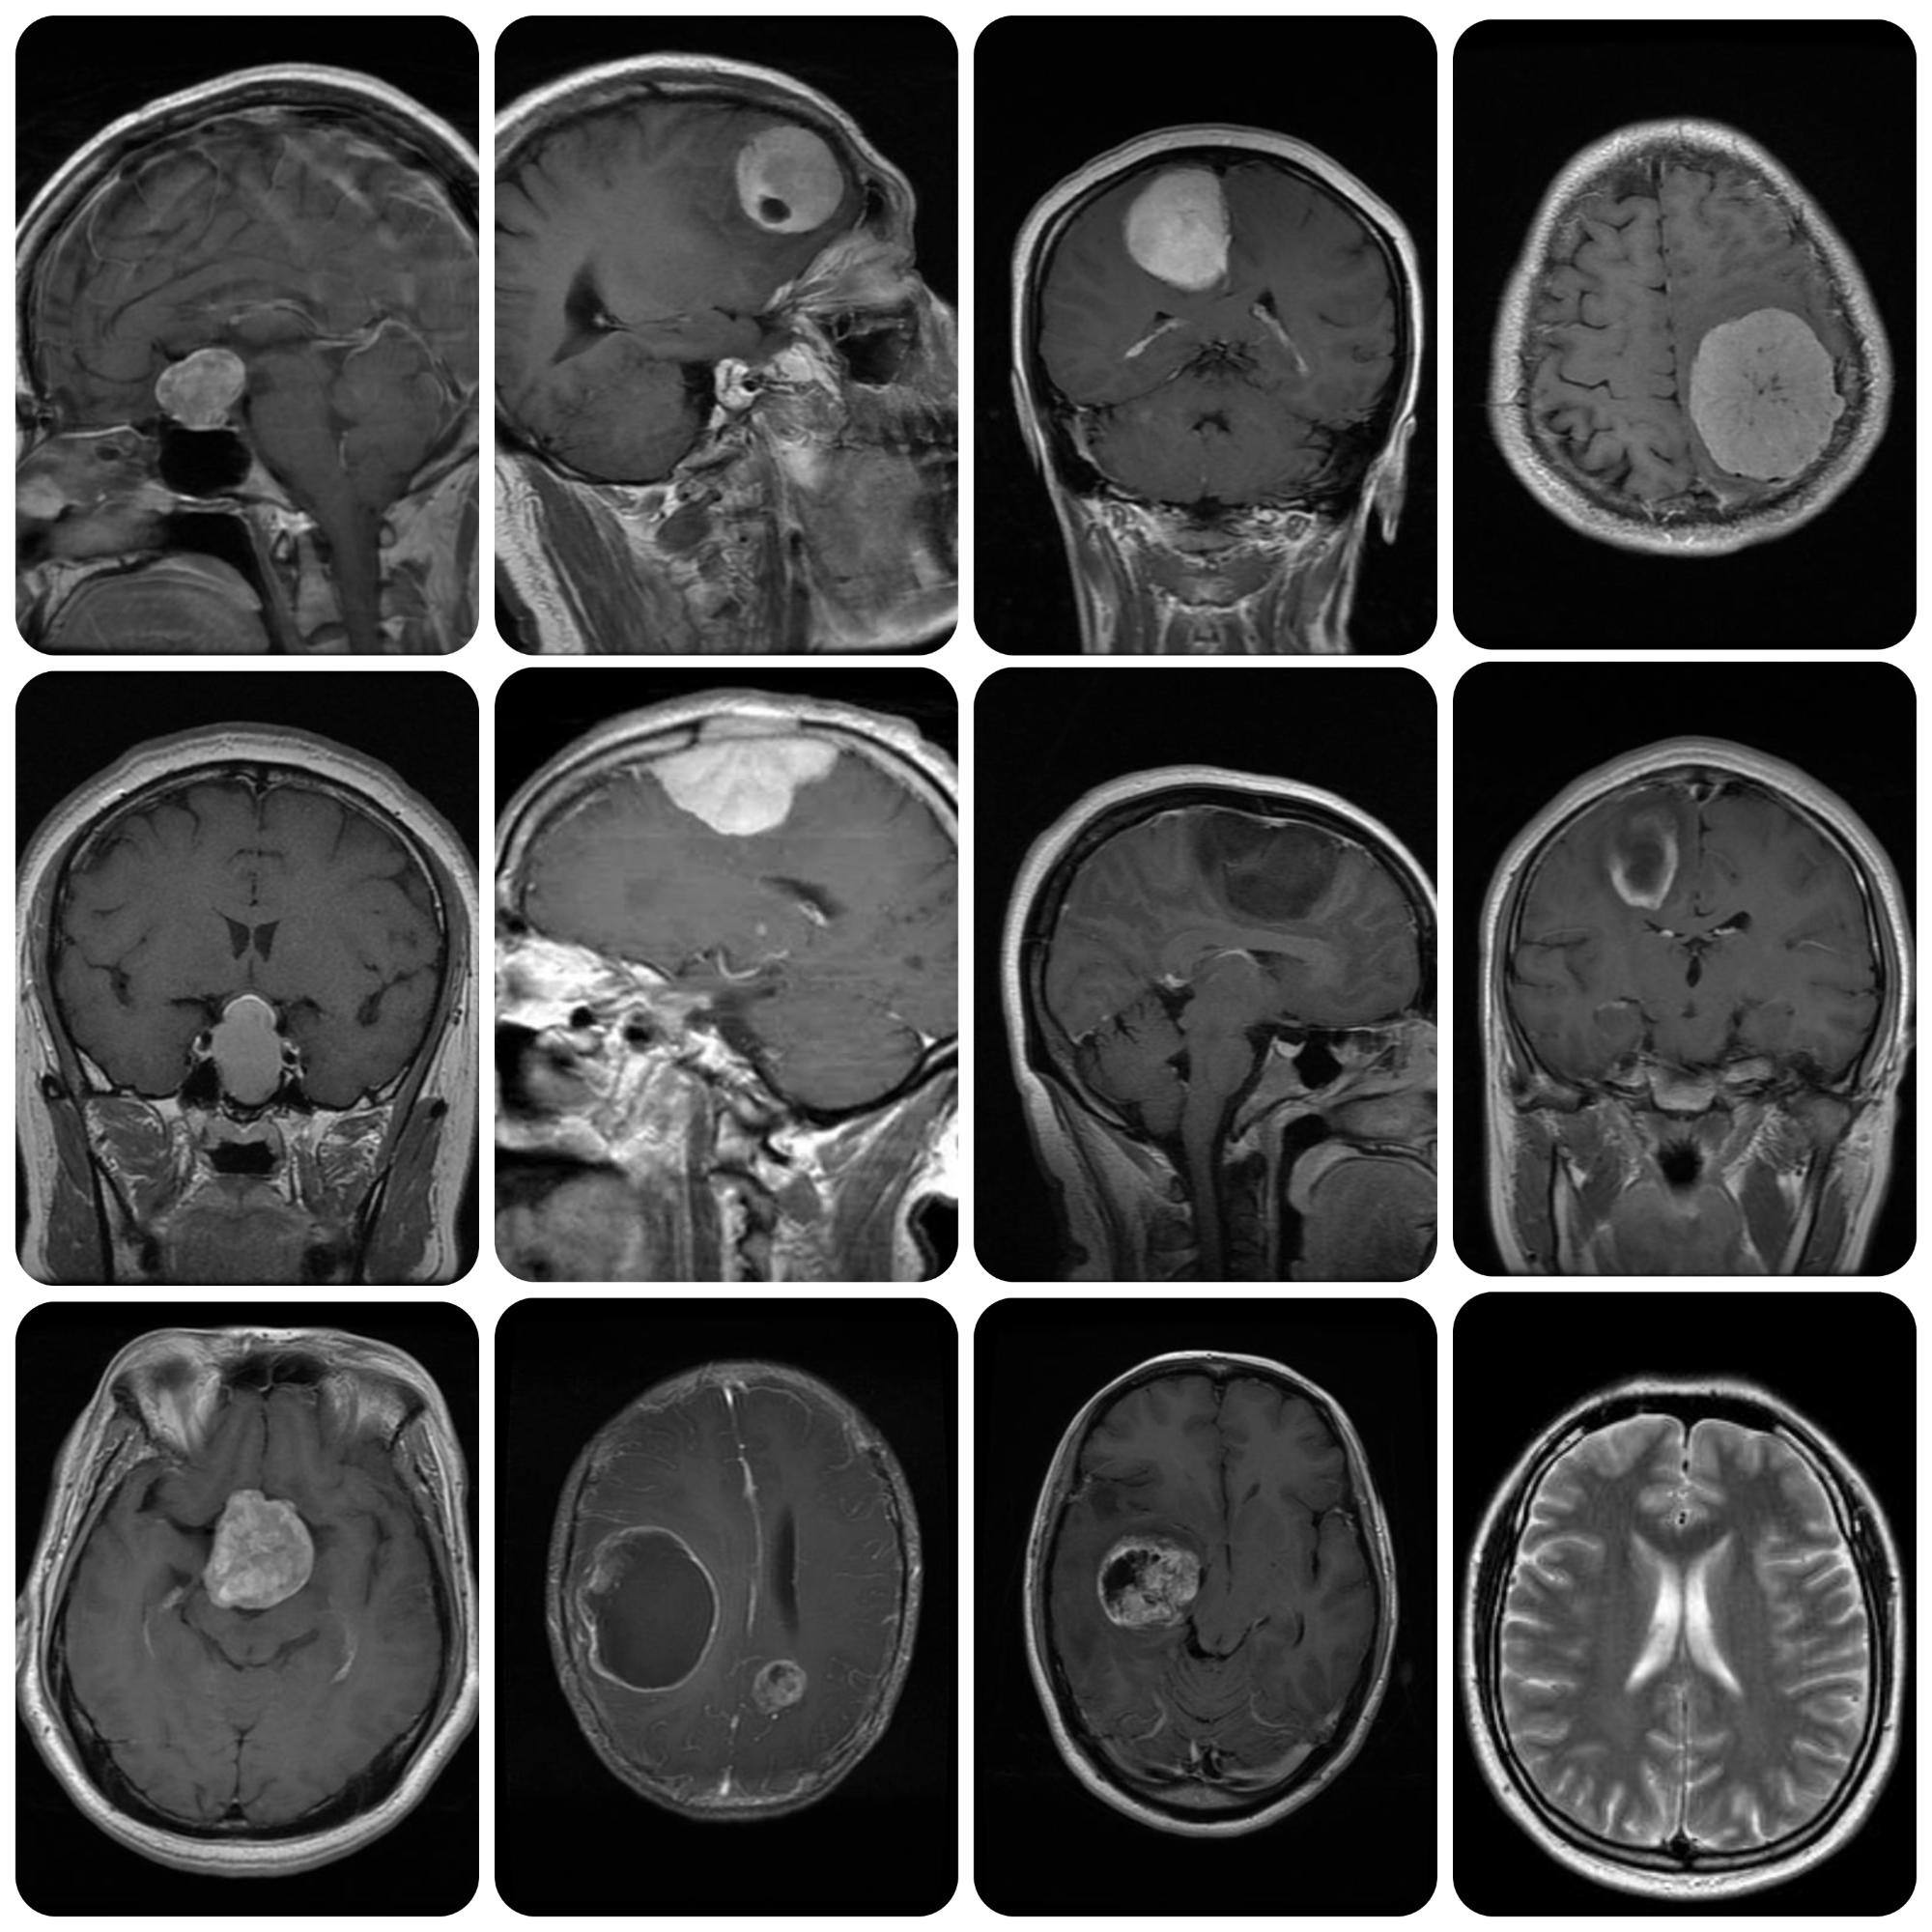
\includegraphics[width=\linewidth]{img/Blank 12 Grids Collage.png}
    \end{subfigure}
    \begin{subfigure}{0.9\textwidth}
        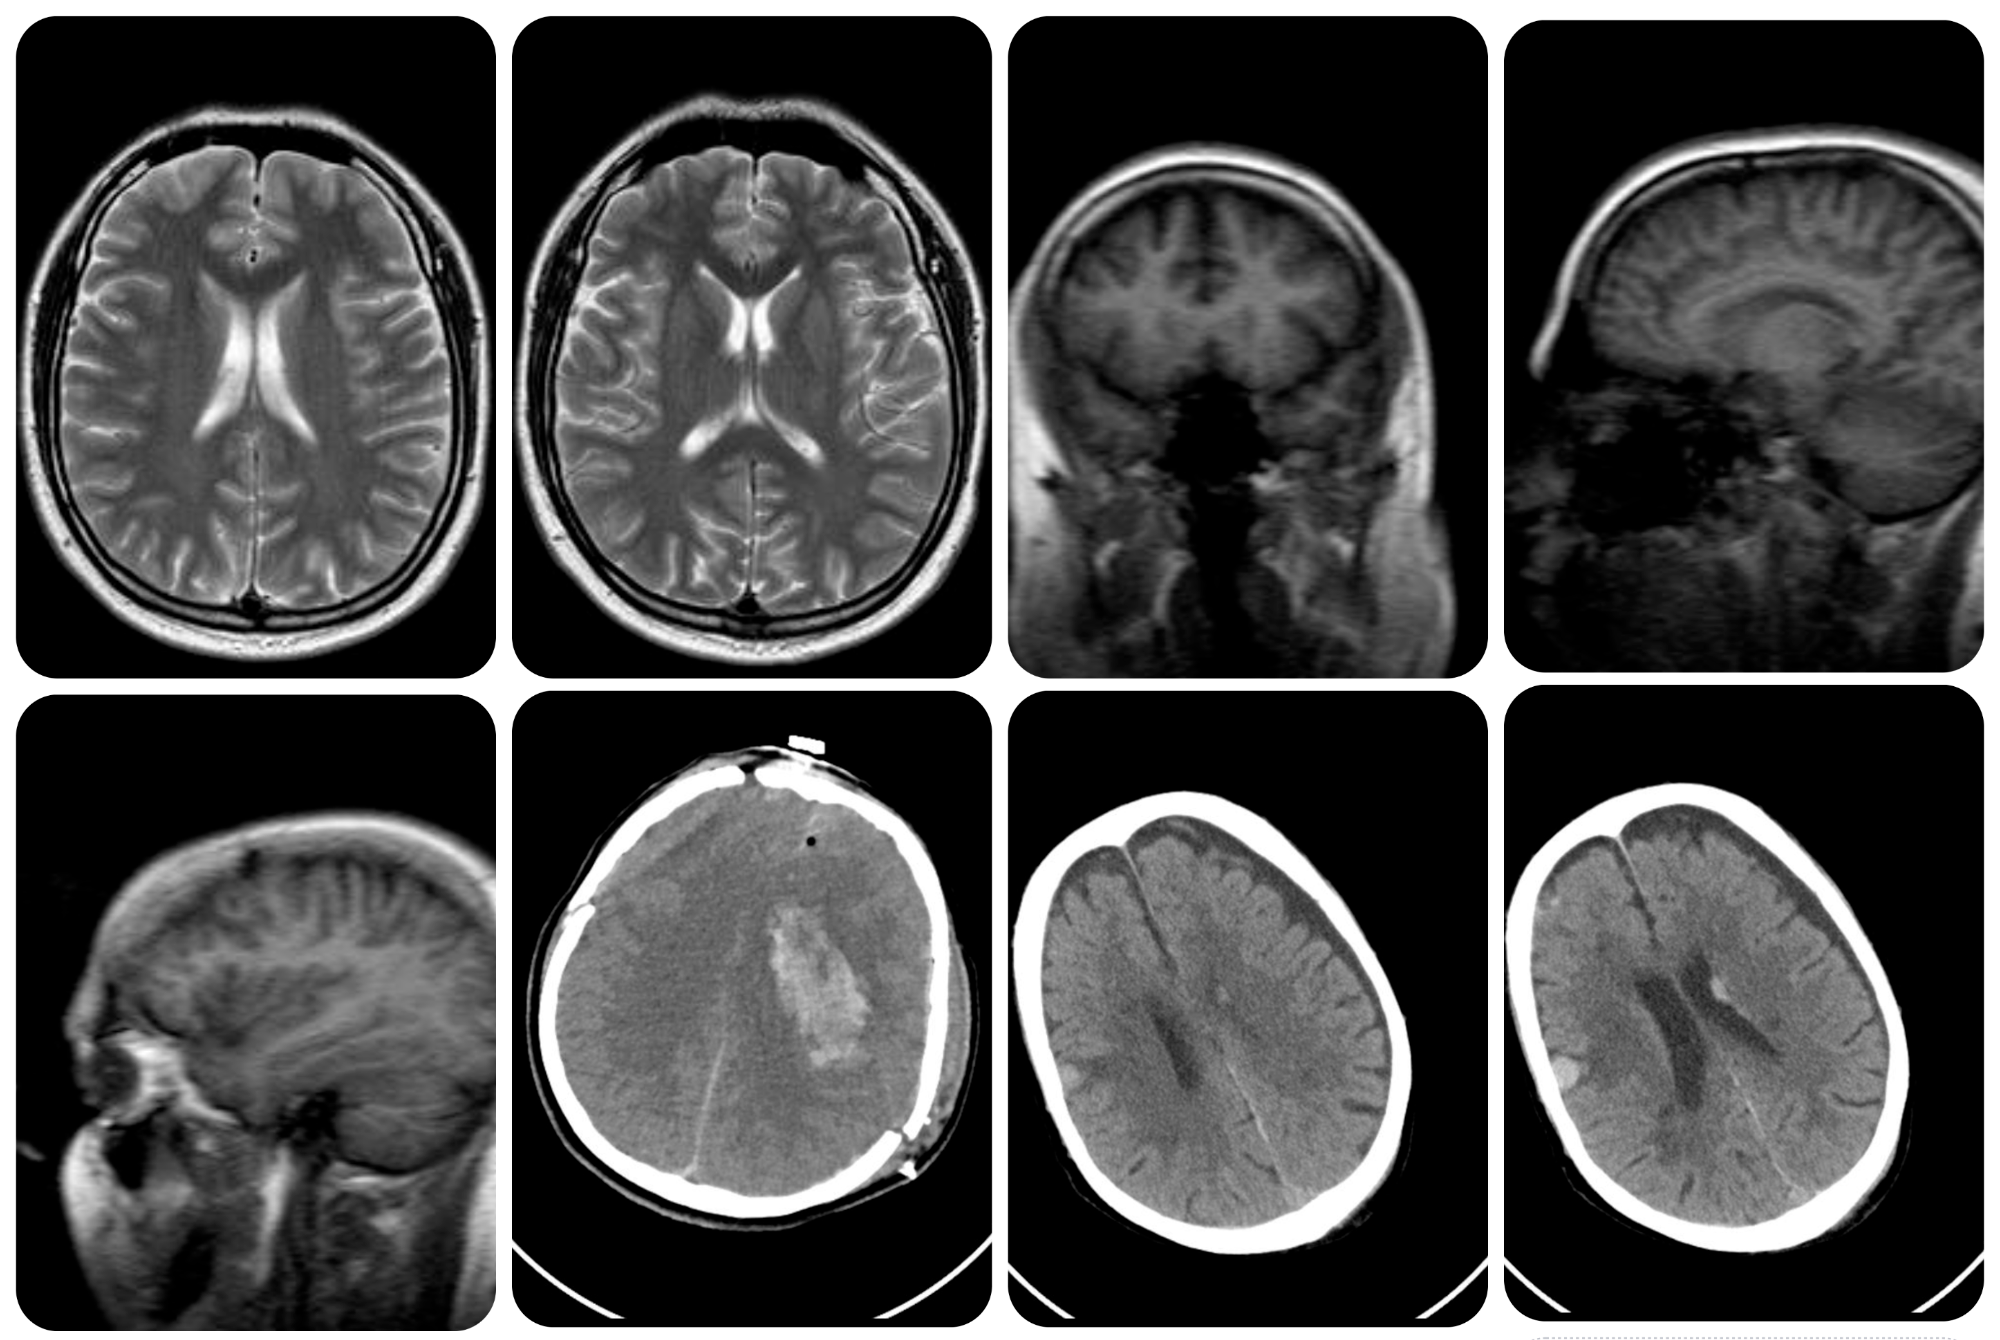
\includegraphics[width=\linewidth]{img/Blank 12 Grids Collage (1).png}
    \end{subfigure}
    \caption{Test images used in the experiments.}
\label{fig:imagenes}    
\end{figure}

The experimental design is multifactorial, focusing on three main factors: the evaluation of the fitness function, the signal-to-noise ratio (PSNR), and the Structural Similarity Index (SSIM). Eight different treatments corresponding to the selected algorithms were carried out: Reptile Search (RSA)~\cite{Abualigah2022}, Orca Predator (OPA)~\cite{Jiang2022}, Honey Badger Algorithm (HBA)~\cite{Hashim2022}, Bald Eagle Search (BES)~\cite{Alsattar2019}, Gray Wolf Optimization (GWO)~\cite{Mirjalili2014}, Crow Search (CSA)~\cite{Askarzadeh2016}, Harris Hawk Optimization (HHO)~\cite{Heidari2019}, and Tuna Swarm Optimization (TSO)~\cite{Xie2021}. The parameters used were tabulated in Table~\ref{tab:algorithms-parameters}, with a population of 30, a set iteration of 100, and 30 independent runs were conducted for each algorithm.

\begin{table}[!t]
	\renewcommand{\arraystretch}{1.3}
	\caption{Algorithms and parameters}
	\label{tab:algorithms-parameters}
	\centering
	\begin{tabular}{|c|c|}
		\hline
		\textbf{Algorithms} & \textbf{parameters} \\
		\hline
		BES                 &                      
		\begin{tabular}{@{}c@{}}
		$c1=c2=2$ \\
		$\alpha=2$ \\
		$a=10$ \\
		$R=1.5$
	\end{tabular} \\
	\hline
	HHO & - \\
	\hline
	OPA &
	\begin{tabular}{@{}c@{}}
		$p1,p2=[0,1]$ \\
		$a=0.01$      
	\end{tabular} \\
	\hline
	CSA &
	\begin{tabular}{@{}c@{}}
		$fl=2$   \\
		$AP=0.1$ 
	\end{tabular} \\
	\hline
	GWO & $a=2$ (linear decreasing) \\
	\hline
	HBA &
	\begin{tabular}{@{}c@{}}
		$\beta=6$ \\
		$C=2$     
	\end{tabular} \\
	\hline
	RSA &
	\begin{tabular}{@{}c@{}}
		$\alpha=0.1$ \\
		$\beta=0.1$  
	\end{tabular} \\
	\hline
	TSO &
	\begin{tabular}{@{}c@{}}
		$z=0.05$ \\
		$a=0.7$  
	\end{tabular} \\
	\hline
	\end{tabular}
\end{table}

\subsection{Activity description}

The primary focus of the research was the in-vivo analysis of the brain using medical image sequences from public datasets. MRI and CT images, which included various brain pathologies, were used to study the effectiveness of segmentation processes. The goal was to achieve the most accurate segmentation of cerebral tissue using advanced optimization methods.

For this purpose, Kapur, Otsu, and Tsallis algorithms, which have been previously validated for their efficacy in segmenting complex anatomical structures in medical images, were applied. These algorithms were tested in our study to determine which provides better results in terms of segmentation accuracy.

Furthermore, an exhaustive analysis was carried out using a Python script, which implemented these algorithms to evaluate the segmentation thresholds in MRI and CT images. Performance metrics such as the PSNR and SSIM were assessed to ensure the quality and accuracy of the segmentation. Each algorithm was executed multiple times to confirm the robustness of the results obtained.

This comprehensive approach not only enhanced the understanding of segmentation techniques applied to specific brain pathologies but also optimized the processes of medical image analysis for future research.

\subsubsection{Validity evaluation}

To ensure the validity of the results obtained in the experimentation with the bioinspired metaheuristic algorithms, several criteria and procedures were established. The validity of the study is addressed from different dimensions: internal validity, which refers to the accuracy with which the treatments reflect variations in the outcomes; external validity, which evaluates the generalization of the results to other contexts; and construct validity, which verifies that the operationalization truly measures the phenomenon under study.

\subsubsection{Internal validity}

For internal validity, extrinsic variables that could influence the performance of the algorithms, such as lighting and quality of the medical images, were controlled. Additionally, the same evaluation protocol was used for all treatments, which includes the optimization function and evaluation indices (PSNR and SSIM). The consistency of the experimental conditions was verified through detailed recording of each step in the algorithm execution procedure.

\subsubsection{External validity}

To ensure external validity, a sample of images from subjects with various brain pathologies was selected, allowing the findings to be extrapolated to a wide range of clinical cases. However, it is acknowledged that further studies are needed to explore the applicability of the algorithms in even more diverse clinical scenarios.

\subsubsection{Construct validity}

Construct validity was ensured through the use of algorithms whose performance has been corroborated in previous research. To strengthen this validity, the performance metrics used (fitness, PSNR, and SSIM) are widely recognized and employed in the field of medical image processing and analysis.

To provide a solid foundation for the evaluation of validity, a pretest of the algorithms and a pilot of the experimental design were conducted on a subset of the sample before full implementation. This allowed for the detection and correction of possible flaws in the proposed methodology. Additionally, the replicability of the research is facilitated by the thorough documentation and availability of the source code used, allowing future studies to verify and build upon our findings.

\subsubsection{Conclusion validity}

To ensure conclusion validity, the Wilcoxon signed-rank test was applied to our algorithm segmentation comparisons. This non-parametric statistical test is ideal for small samples or data that do not distribute normally. A significance level was set a priori, and the effect size was evaluated to determine the practical relevance of the results. By controlling for Type I and II errors, we ensured the statistical robustness of our conclusions, limiting the possibility of misinterpretations of the treatment effect.

\subsection{Data analysis definition}

In the data analysis phase of our study, the main statistical approach employed will be the Friedman test. This non-parametric test will be used to evaluate differences in performance metrics —fitness, Structural Similarity (SSIM), and Signal-to-Noise Ratio (PSNR)— among the various segmentation algorithms applied to the dataset of medical images.

Each metric will be analyzed independently using this test to identify if the improvements obtained by the different algorithms are statistically significant. Statistical significance will be established with a predefined p-value. Additionally, the effect size will be calculated for each comparison to quantify the magnitude of the observed differences.

Upon concluding the analysis, the results will provide a detailed perspective on the relative performance of each algorithm, facilitating the identification of the most effective methods for in-vivo brain segmentation.


\section{Metaheuristic Algorithms} \label{sec:mh} 

In this section, multilevel thresholding is performed using metaheuristic algorithms by maximizing Kapur's entropy ~\ref{eq_Kapur}, Otsu's method ~\ref{eq_Otsu}, and Tsallis's entropy ~\ref{eq_Tsallis} as follows:

\begin{equation}
\begin{gathered}
\max(F_{kapur}(th)) \
\text{th} \in 0 \leq \text{th}_i \leq 255
\end{gathered}
\label{eq_Kapur}
\end{equation}

\noindent 
where $i=[1,2,...,n]$, with $n$ being the number of thresholds.

\begin{equation}
\begin{gathered}
\max(\sigma_B^2(th)) \
\text{th} \in 0 \leq \text{th} \leq 255
\end{gathered}
\label{eq_Otsu}
\end{equation}
\begin{equation}
\begin{gathered}
\max(J_{Tsallis}(\mathbf{t})) \
\mathbf{t} = (t_1, t_2, \dots, t_k) \in \mathbb{Z}^k \
0 \leq t_i \leq 255, \quad i = 1, 2, \dots, k
\end{gathered}
\label{eq_Tsallis}
\end{equation}

\noindent 
where $J_{Tsallis}(\mathbf{t})$ is the Tsallis entropy for a given threshold vector $\mathbf{t}$, defined as:

\begin{equation}
J_{Tsallis}(\mathbf{t}) = \sum_{i=1}^{k+1} \frac{w_i}{w_T} S_i + (1-q) \prod_{i=1}^{k+1} S_i
\end{equation}

\noindent 
with $S_i$ being the Tsallis entropy for region $i$:

\begin{equation}
S_i = \frac{1}{q-1}\left(1 - \sum_{p=l_i}^{u_i} \left(\frac{h(p)}{w_i}\right)^q\right)
\end{equation}

\noindent 
and $q$ is the non-extensivity parameter, $l_i$ and $u_i$ are the lower and upper limits of region $i$, $w_i$ is the weight of region $i$, $h(p)$ is the normalized histogram for pixel value $p$, and $w_T$ is the total weight of the image.
The metaheuristic algorithms aim to find the optimal threshold vector $\mathbf{t}^*$ that maximizes the Tsallis entropy:

\begin{equation}
\mathbf{t}^* = \arg\max_{\mathbf{t}} J_{Tsallis}(\mathbf{t})
\end{equation}

Here, $\sigma_B^2(th)$ represents the between-class variance for a threshold $th$, and the objective is to find the value of $th$ that maximizes this variance, with $th$ varying in the range of 0 to 255 for 8-bit grayscale images.

\subsection{Bald Eagle Search}

The Bald Eagle Search (BES) algorithm, proposed by Alsattar et al.~\cite{Alsattar2019}, is a bio-inspired metaheuristic algorithm that mimics the hunting strategy or intelligent social behavior of bald eagles while hunting fish.

The area identification stage relates to the bald eagle when it performs a search for the best position $P$ to hunt for food (select space). This stage is mathematically represented as:

\begin{equation}
\begin{gathered}
P_{new}=P_{best}+{\alpha}r(P_{mean}-P_{i})\\
\end{gathered}
\label{eq11}
\end{equation}

Once the best position in space is selected, the bald eagle performs different spiral movements to increase the speed of the food search process. This stage is called search within the area (search space) and is mathematically represented as:

\begin{equation}
\begin{gathered}
P_{new}=P_{i}+y(i)(P_{i}-P_{i+1})+x(i)(P_{i}-P_{mean}) \\
x(i)= \frac{xr_{i}}{max(\lvert xr \rvert)} ~\ , ~\ y(i)= \frac{yr_{i}}{max(\lvert yr \rvert)} \\
xr(i)=r(i)\cdot \sin (\theta(i)) ~\ , ~\ yr(i)=r(i)\cdot \cos (\theta(i)) \\
\theta(i)=a\cdot r\cdot rnd ~\ , ~\ r(i)=\theta(i)+R \cdot rnd 
\end{gathered}
\label{eq12}
\end{equation}

The last stage of the BES algorithm corresponds to the selection and attack of the prey, called swoop. The swoop consists of moving all the best points towards the target. Mathematically, this is expressed as:

\begin{equation}
\begin{gathered}
P_{\text{new}} = \text{rnd} \cdot P_{\text{best}} + x1(i)(P_{i}-c1 \cdot P_{\text{mean}}) \\
+ y1(i)(P_{i}-c2 \cdot P_{\text{best}}) \\
x1(i) = \frac{xr_{i}}{\max(\lvert xr \rvert)}, \quad y1(i) = \frac{yr_{i}}{\max(\lvert yr \rvert)} \\
xr(i) = r(i) \cdot \sinh(\theta(i)), \quad yr(i) = r(i) \cdot \cosh(\theta(i))
\end{gathered}
\end{equation}

\subsection{Harris hawk optimization}

The Harris Hawk Optimization (HHO) algorithm is a bio-inspired algorithm proposed by Heidari et al.~\cite{Heidari2019} based on the behavior of Harris Hawks. The algorithm was modeled through the exploration and exploitation phases. In the exploration phase, the Harris Hawk can detect and track its prey with its powerful eyes. In HHO, the Harris Hawk can randomly stay in some locations and wait to detect prey based on its strategy. If an equal chance $q$ is considered for each perched strategy based on the position of family members, it can be modeled as a condition $q<0.5$, or perched at a random position in the trees as $q\geq 0.5$, as shown:

\begin{equation}
\begin{gathered}
X(t+1)= \\
\begin{cases}
  X_{rnd}(t) - r_1 |X_{rnd}(t) -2 r_2 X(t)| , q \geq 0.5 \\
  X_{rab}(t) - X_m(t) - r3(LB + r_4 (UB-LB)) , q < 0.5
\end{cases}
\end{gathered}
\end{equation}

The average position can be calculated by:

\begin{equation}
X_m (t) = \frac{1}{N} \sum_{i=1}^{N} X_i(t) 
\label{eq14}
\end{equation}

In the transition from exploration to exploitation, when prey escapes, it loses energy. This loss is modeled as:

\begin{equation}
E = 2 E_0 (1 - \frac{t}{T}) 
\label{eq15}
\end{equation}

The parameter $E$ indicates the escape energy of the prey, and $T$ is the maximum number of iterations. On the other hand, $E_0$ is a random parameter that oscillates between $(-1,1)$ for each iteration.

The exploitation phase is divided into soft besiege and hard besiege. In soft besiege, the conditions $r \geq 0.5$ and $|E| \geq 0.5$ must be met. The prey tries to escape through some random jumps but finally fails. This is modeled as:

\begin{equation}
\begin{gathered}
X(t+1) = \Delta X(t) - E |J X_{rabb}(t) -X(t)| \\
\Delta X(t) = X_{rabb}(t) - X(t)
\end{gathered}
\label{eq16}
\end{equation}

In hard besiege, $r \geq 0.5$ and $|E| < 0.5$ must be met. The prey is too tired to escape. In this case, the position is updated according to:

\begin{equation}
\begin{gathered}
X(t+1) = X_{rabb}(t) - E |\Delta X(t)| \\
\end{gathered}
\label{eq17}
\end{equation}

\subsection{Orca predator algorithm}

The Orca Predator Algorithm (OPA), proposed by Jiang et al.~\cite{Jiang2022}, is a metaheuristic algorithm bio-inspired by the behavior of Orcas. Orcas are highly intelligent carnivorous beings in the dolphin family. They live in families with approximately 30 members. Orcas communicate with each other through sounds, coordinating their movements to herd fish, drive them to the surface, and finally encircle them. The Orca group model can swim in $1-D, 2-D, 3-D$ or in an extra-dimensional space. This is defined as:

\begin{equation}
\begin{gathered}
X = [ x1, x2, ..., xN ] =\begin{bmatrix}
  x1,1 & x1,2 & ... & x1,D  \\
  x2,2 & x2,2 & ... & x2,D  \\
  \vdots & \vdots & \vdots & \vdots \\
  xN,1 & xN,2 & ... & xN,D
\end{bmatrix}
\end{gathered}
\label{eq18}
\end{equation}

The movement of Orcas herding fish can be modeled by the movement velocity as follows:

\begin{equation}
\begin{gathered}
v_{chase,1,i}^t = a ( d x_{best}^t - F (b M^t + c x_i^t)) \\
v_{chase,2,i}^t = e x_{best}^t - x_{i}^t \\
M = \frac{\sum_{i=1}^{N} x_i^t}{N} \\
c=1-b \\
\begin{cases}
  x_{chase,1,i}^t = x_{i}^t + v_{chase,1,i}^t , \text{if} \;rand > q \\
  x_{chase,2,i}^t = x_{i}^t + v_{chase,2,i}^t  , \text{if} \;rand \leq q
\end{cases}
\end{gathered}
\label{eq19}
\end{equation}

The herding of prey is performed by the position of three randomly selected Orcas, and then their position can be determined as:

\begin{equation}
\begin{gathered}
x_{chase,3,i}^t =x_{j1,k}^t +u \times (x_{j2,k}^t - x_{j3,k}^t ) \\
u = 2 \times (\text{rand} - \frac{1}{2}) \times \frac{Max_{iter}-t}{Max_{iter}}
\end{gathered}
\label{eq20}
\end{equation}

The position adjustment is determined by comparing the best values obtained in the fitness function, modeled as:

\begin{equation}
\begin{gathered}
\begin{cases}
  x_{chase,i}^t = x_{chase,i}^t \;\;, \text{if} \; f(x_{chase,i}^t) < f(x_{i}^t ) \\
  x_{chase,t}^t = x_{i}^t  \;\;, \text{if} \;f(x_{chase,i}^t) \geq f(x_{i}^t )
\end{cases}
\end{gathered}
\label{eq21}
\end{equation}

\noindent 
where $f(x_{chase,i}^t)$ corresponds to the value of the fitness function at $x_{chase,i}^t$, and $f(x_{i}^t )$ corresponds to the value of the fitness function at $x_{i}^t$.

\subsection{Crow search algorithm}

The Crow Search Algorithm (CSA), originally proposed by Askarzadeh et al.~\cite{Askarzadeh2016}, is a metaheuristic algorithm bio-inspired by the behavior of Crows. Crows are considered the most intelligent birds. They observe other birds, noting where they hide their food, and steal it when they are not around. In fact, they use their own experience of having been thieves to predict the behavior of a thief and can determine the safest path to protect their treasures against theft. The first step is associated with position and is modeled as:

\begin{equation}
\begin{gathered}
x^{i,iter} = [x_{1}^{i,iter}, x_{2}^{i,iter},...,x_{d}^{i,iter}]\\
x^{i,iter+1}=x^{i,iter}+r_{i} \times fl^{i,iter} \times (m^{j,iter}-x^{i,iter})
\end{gathered}
\label{eq23}
\end{equation}

Crow $j$ knows that crow $i$ is following it. As a result, to protect its cache against theft, crow $j$ deceives crow $i$ by going to another position in the search space. This is modeled as:

\begin{equation}
\begin{gathered}
x^{i,iter+1}=\\
\begin{cases}
x^{i,iter}+r_{i} fl^{i,iter} (m^{j,iter} - x^{i,iter}) \; \; \; r_j \geq AP^{i,iter}\\
\text{a random position} \; \; \; \; \; \;\; \; \;\; \; \;\;\; \; \;\;\; \; \; \; \;\;\; \; \;\; \; \;  \text{otherwise}
\end{cases}
\end{gathered}
\label{eq24}
\end{equation}

\subsection{Gray wolf optimization}

The Gray Wolf Optimization (GWO) algorithm, originally proposed by Mirjalili et al.~\cite{Mirjalili2014}, is a metaheuristic algorithm bio-inspired by the behavior of Gray Wolves. Gray Wolves are considered super predators, living in packs with group sizes ranging from 5 to 12 individuals. Mathematically, a hierarchy within the pack is considered, where the values of the solutions are stored in order, in $\alpha$, $\beta$, and $\delta$, as first, second, and third, respectively. The remaining solutions are stored in $\omega$. The GWO algorithm stores the hunt guided by $\alpha,\beta$ and $\delta$ while $\omega$ follows the other variables.

The hunting phase begins with encircling the prey, modeled as:

\begin{equation}
\begin{gathered}
\vec{D} = |\vec{C} \times \vec{X_p}(t)-\vec{X}(t)|\\
\vec{X}(t+1) = \vec{X_p}(t) - \vec{A} \times \vec{D}
\end{gathered}
\label{eq25}
\end{equation}

\noindent 
where $\vec{A}$ and $\vec{C}$ are vector coefficients, and $\vec{X}$ is the position. The hunt is guided by the alpha, while beta and delta do not usually participate. Mathematically, it is assumed that alpha, beta, and delta have the best knowledge about the position of the prey. Then, the three best solutions are stored, and the other agents are forced to move and update their positions according to the best solutions.

\begin{equation}
\begin{gathered}
\vec{D}_{\alpha} = |\vec{C}_1 \times \vec{X}_{\alpha} -\vec{X}|, \vec{D}_{\beta} = |\vec{C}_1 \times \vec{X}_{\beta} -\vec{X}| \\
\vec{D}_{\delta} = |\vec{C}_1 \times \vec{X}_{\delta} -\vec{X}|\\
\vec{X}_1=\vec{D}_{\alpha}-\vec{A}_1 \times (\vec{D}_{\alpha}), \vec{X}_2=\vec{D}_{\beta}-\vec{A}_2 \times (\vec{D}_{\beta})\\
\vec{X}_3=\vec{D}_{\delta}-\vec{A}_3 \times (\vec{D}_{\delta}) \\
\vec{X}(t+1) = \frac{\vec{X}_1+\vec{X}_2+\vec{X}_3}{3}
\end{gathered}
\label{eq26}
\end{equation}

\subsection{Honey badger algorithm}

The Honey Badger Algorithm (HBA), originally proposed by Hashim et al.~\cite{Hashim2022}, is a bioinspired metaheuristic algorithm based on the behavior of the honey badger. The honey badger follows the honey guide bird, and can also smell and dig at locations where honey is present. The honey guide bird lacks the ability to dig for honey, whereas the honey badger can dig, and it is common for both the honey guide bird and the honey badger to share the reward. The population of candidate solutions is modeled as:

\begin{equation}
\begin{gathered}
\text{Population of candidate solutions}=\\\begin{bmatrix}
  x1,1 & x1,2 & ... & x1,D  \\
  x2,2 & x2,2 & ... & x2,D  \\
  \vdots & \vdots & \vdots & \vdots \\
  xn,1 & xn,2 & ... & xn,D
\end{bmatrix}
\end{gathered}
\label{eq27}
\end{equation}

The intensity is related to the concentration power of the prey and the distance between the prey and the $ith$ honey badger. The intensity of the prey's scent is represented by $I_i$, where a high scent intensity leads to faster movement and vice versa. This is defined as:

\begin{equation}
\begin{gathered}
I_1 = r_2 \times \frac{S}{4 \pi d_i^2}\\
S = (x_i - x_{i+1})^2\\
d_i = x_{prey} - x_i
\end{gathered}
\label{eq28}
\end{equation}

\noindent 
where $S$ represents the concentration power, $d_i$ denotes the distance between the prey and the $ith$ honey badger. Additionally, the density factor $\alpha$ controls the randomization of the time-variant to ensure a transition from exploration to exploitation, as shown:

\begin{equation}
\begin{gathered}
\alpha = C \times exp\left(-\frac{t}{t_{max}}\right)\\
\end{gathered}
\label{eq29}
\end{equation}

In the digging phase, the honey badger performs a cardioid movement, as follows:

\begin{equation}
\begin{gathered}
x_{new} = x_{prey} + F \times \beta \times I \times x_{prey} + \\
F \times r_3 \times \alpha \times d_i \times \left|\cos(2\pi r_4) \times [1-\cos(2\pi r_5)]\right|
\end{gathered}
\label{eq30}
\end{equation}

\noindent 
where $x_{prey}$ corresponds to the position of the prey, $r_3$, $r_4$, and $r_5$ are random numbers between 0 and 1. $F$ acts as a flag that alters the search direction, as follows:

\begin{equation}
\begin{gathered}
F=
\begin{cases}
1, & \text{if } r_6 \leq 0.5 \\
-1, & \text{otherwise}
\end{cases}
\end{gathered}
\label{eq31}
\end{equation}    

\noindent 
where $r_6$ is a random number between 0 and 1. Finally, the position is updated by the honey guide bird, which can be simulated as:

\begin{equation}
\begin{gathered}
x_{new} = x_{prey} + F \times r_7 \times \alpha \times d_i
\end{gathered}
\label{eq32}
\end{equation}

\noindent 
where $r_7$ is a random number between 0 and 1.

\subsection{Reptile search algorithm}

The Reptile Search Algorithm (RSA), originally proposed by Abualigah et al.~\cite{Abualigah2022}, is based on the behavior of crocodiles during hunting. 

\begin{equation}
\begin{gathered}
X = \begin{bmatrix}
  x1,1 & x1,2 & ... & x1,n  \\
  x2,2 & x2,2 & ... & x2,n  \\
  \vdots & \vdots & \vdots & \vdots \\
  xN,1 & xN,2 & ... & xN,n
\end{bmatrix}
\end{gathered}
\label{eq33}
\end{equation}

he exploration phase is defined by:

\begin{equation}
\begin{gathered}
x_{(i,j)}(t+1)=\\
\begin{cases}
Best_j (t) - \eta_{(i,j)} \times \beta - R_{(i,j)}(t) \times rand, & t \leq \frac{T}{4} \\
Best_j (t) \times x_{(r_1,j)} \times ES(t) \times rand, & t \leq 2\frac{T}{4} and t \geq \frac{T}{4} \\
\end{cases}
\end{gathered}
\label{eq34}
\end{equation}   

\begin{equation}
\begin{gathered}
\eta_{(i,j)} = Best_j(t) \times P_{(i,j)}
\end{gathered}
\label{eq35}
\end{equation}

\begin{equation}
\begin{gathered}
R_{(i,j)} = \frac{Best_j(t) - x_{(r_2,j)}}{Best_j(t) + \epsilon}
\end{gathered}
\label{eq36}
\end{equation}

\begin{equation}
\begin{gathered}
ES(t) = 2 \times r_3 \times (1 - \frac{1}{T})
\end{gathered}
\label{eq37}
\end{equation}

\begin{equation}
\begin{gathered}
P_{(i,j)} = \alpha + \frac{x_{(i,j) - M(x_i)}}{Best_j(t) \times (UB_{(j)}-LB_{(j)}) + \epsilon} 
\end{gathered}
\label{eq38}
\end{equation}

\begin{equation}
\begin{gathered}
M_{(x_i)} = \frac{1}{n} \sum_{j=1}^{n} x_{(i,j)}
\end{gathered}
\label{eq39}
\end{equation}

\subsection{Tuna swarm optimization}

The Tuna Swarm Optimization (TSO), proposed by Xie et al.~\cite{Xie2021}, is inspired by the foraging strategies of tunas, which include spiral and parabolic formations for hunting prey.

\subsubsection{Initialization}

The initialization of TSO is performed by generating initial populations randomly and uniformly within the search space:

\begin{equation}
    \begin{gathered}
        X_{\text{init}} = \\
        \text{rand} \cdot (ub - lb) + lb, \quad i = 1, 2, ..., NP
    \end{gathered}
\end{equation}

\noindent 
where $X_{\text{init}}$ is the $i$-th initial individual, $ub$ and $lb$ are the upper and lower bounds of the search space, $NP$ is the number of tuna populations, and $\text{rand}$ is a uniformly distributed random vector from 0 to 1.

\subsubsection{Spiral foraging}

Spiral foraging is modeled as follows, adjusting the position of tunas towards an optimum point or a random reference point based on the phase of the iteration:

\begin{equation}
    \begin{gathered}
        X_{t+1}^i = \\
        \quad
        \begin{cases}
            \alpha_1 \cdot \left(X_{\text{best}}^t + \beta \cdot \left\lVert X_{\text{best}}^t - X_t^i \right\rVert \right) + \alpha_2 \cdot X_t^i, & \text{if } i = 1,\\
            \alpha_1 \cdot \left(X_{\text{rand}} + \beta \cdot \left\lVert X_{\text{rand}} - X_t^i \right\rVert \right) + \alpha_2 \cdot X_t^{i-1}, & \text{if } i = 2,3,...,NP,
        \end{cases}
    \end{gathered}
\end{equation}

\noindent 
where $\alpha_1$, $\alpha_2$ are weighting coefficients, $\beta$ involves a random variable $b$, and $X_{\text{rand}}$ is a random reference point.

\subsubsection{Parabolic foraging}

Parabolic foraging is described as:

\begin{equation}
    \begin{gathered}
        X_{t+1}^i = \\
        \begin{cases}
            X_{\text{best}}^t + \text{rand} \cdot (X_{\text{best}}^t - X_t^i) + TF \cdot p^2 \cdot (X_{\text{best}}^t - X_t^i), & \text{if rand } < 0.5,\\
            TF \cdot p^2 \cdot X_t^i, & \text{if rand } \geq 0.5,
        \end{cases}
    \end{gathered}
\end{equation}

\noindent 
where $TF$ is a random number with a value of 1 or -1, and $p$ is a probability that varies with the iteration.

These strategies enable TSO to perform effective global exploration and precise local exploitation of the search space. Individuals in the algorithm alternate between spiral and parabolic foraging strategies, adapting their behavior to find optimal solutions.

In the evaluations conducted using the Kapur, Otsu, and Tsallis objective functions, GWO and TSO consistently outperformed the others, demonstrating the highest effectiveness across all objective functions. HBA and OPA also showed strong performance, though they generally ranked just below GWO and TSO in terms of overall effectiveness. Conversely, RSA and BES exhibited the poorest performance across all tests, consistently ranking at the bottom.

The analysis conducted using the Friedman test with the Kapur objective function and the SSIM metric revealed that GWO was the most consistently effective algorithm, achieving average rankings between 1.3 and 2.1. HBA followed closely, with rankings ranging from 2.15 to 3.05. Intermediate performance was observed for OPA, CSA, and HHO, while RSA, BES, and TSO recorded the lowest rankings across all evaluated dimensions. This trend remained stable throughout the analysis, indicating a clear hierarchy in the efficacy of the algorithms.

\begin{figure}[H] \centering 
\includegraphics[width=0.8\textwidth]{SSIM/Kapur/Metrica_kapur_Friedman_results.png} \caption{Average Rank of the SSIM metric by dimension K, Kapur entropy objective function} \label{fig
} \end{figure}

When evaluating the SSIM metric across dimensions 7, 8, and 9, the OPA algorithm consistently achieved the highest rankings, with values ranging from 2.3 to 2.7. GWO also demonstrated robust performance, with rankings between 2.45 and 3.05. HBA and CSA occupied intermediate positions, while RSA, BES, HHO, and TSO consistently recorded the lowest rankings. OPA emerged as the most effective algorithm for the Otsu objective function according to the SSIM metric, with GWO following closely.

\begin{figure}[H] \centering 
\includegraphics[width=0.8\textwidth]{SSIM/Otsu/Metrica_Otsu_Friedman_results.png} \caption{Average Rank of the SSIM metric by dimension K, Otsu objective function} \label{fig
} \end{figure}

The Friedman test results for the Tsallis objective function and the SSIM metric across dimensions 7, 8, and 9 revealed significant performance differences among the algorithms. CSA consistently achieved the best average rankings, ranging from 1.15 to 1.35, closely followed by GWO, which maintained rankings between 3.0 and 3.2. HBA and OPA performed at intermediate levels. Overall, CSA demonstrated the best performance for the Tsallis objective function according to the SSIM metric, with GWO following, while RSA, BES, HHO, and TSO recorded the lowest rankings.

\begin{figure}[H] \centering 
\includegraphics[width=0.8\textwidth]{SSIM/Tsallis/Metrica_Tsallis_Friedman_results.png} \caption{Average Rank of the SSIM metric by dimension K, Tsallis objective function} \label{fig
} \end{figure}

The analysis of the results using the Friedman-Kapur test indicated that OPA consistently achieved the best average rank, with a value of 2.2, across the different K dimensions. BES and TSO consistently showed the poorest performance, with rankings ranging from 7.2 to 7.8, making them the least effective algorithms evaluated.

\begin{figure}[H] \centering 
\includegraphics[width=0.8\textwidth]{PSNR/Kapur/Metrica_kapur_Friedman_results.png} \caption{Average Rank of the PSNR metric by dimension K, Kapur entropy objective function} \label{fig
} \end{figure}

The results of the analysis showed that OPA exhibited the best performance according to the PSNR metric, followed by RSA. In contrast, BES and TSO consistently obtained the highest ranks, indicating the poorest performance across the evaluated dimensions.

\begin{figure}[H] \centering 
\includegraphics[width=0.8\textwidth]{PSNR/Otsu/Metrica_Otsu_Friedman_results.png} \caption{Average Rank of the PSNR metric by dimension K, Otsu objective function} \label{fig
} \end{figure}

The analysis results for the Tsallis objective function and the PSNR metric indicate that CSA, HBA, and GWO consistently delivered the best performances across the different dimensions, with CSA standing out as the top performer. On the other hand, BES, HHO, and TSO recorded the lowest performance levels in most of the evaluated dimensions.

\begin{figure}[H] \centering 
\includegraphics[width=0.8\textwidth]{PSNR/Tsallis/Metrica_Tsallis_Friedman_results.png} \caption{Average Rank of the PSNR metric by dimension K, Tsallis objective function} \label{fig
} \end{figure}

The analysis identified that GWO and TSO demonstrated outstanding performance in the context of the Kapur objective function. GWO recorded an exceptionally low average rank of 1.1 in dimension 7 and maintained strong performance across all three dimensions. TSO also exhibited remarkable consistency, with a rank of 1.9 in dimension 7 and the best ranks of 1.95 in dimensions 8 and 9, underscoring the effectiveness of both algorithms in this specific context. RSA, BES, and OPA, on the other hand, showed the poorest performance according to the fitness metric.

\begin{figure}[H] \centering 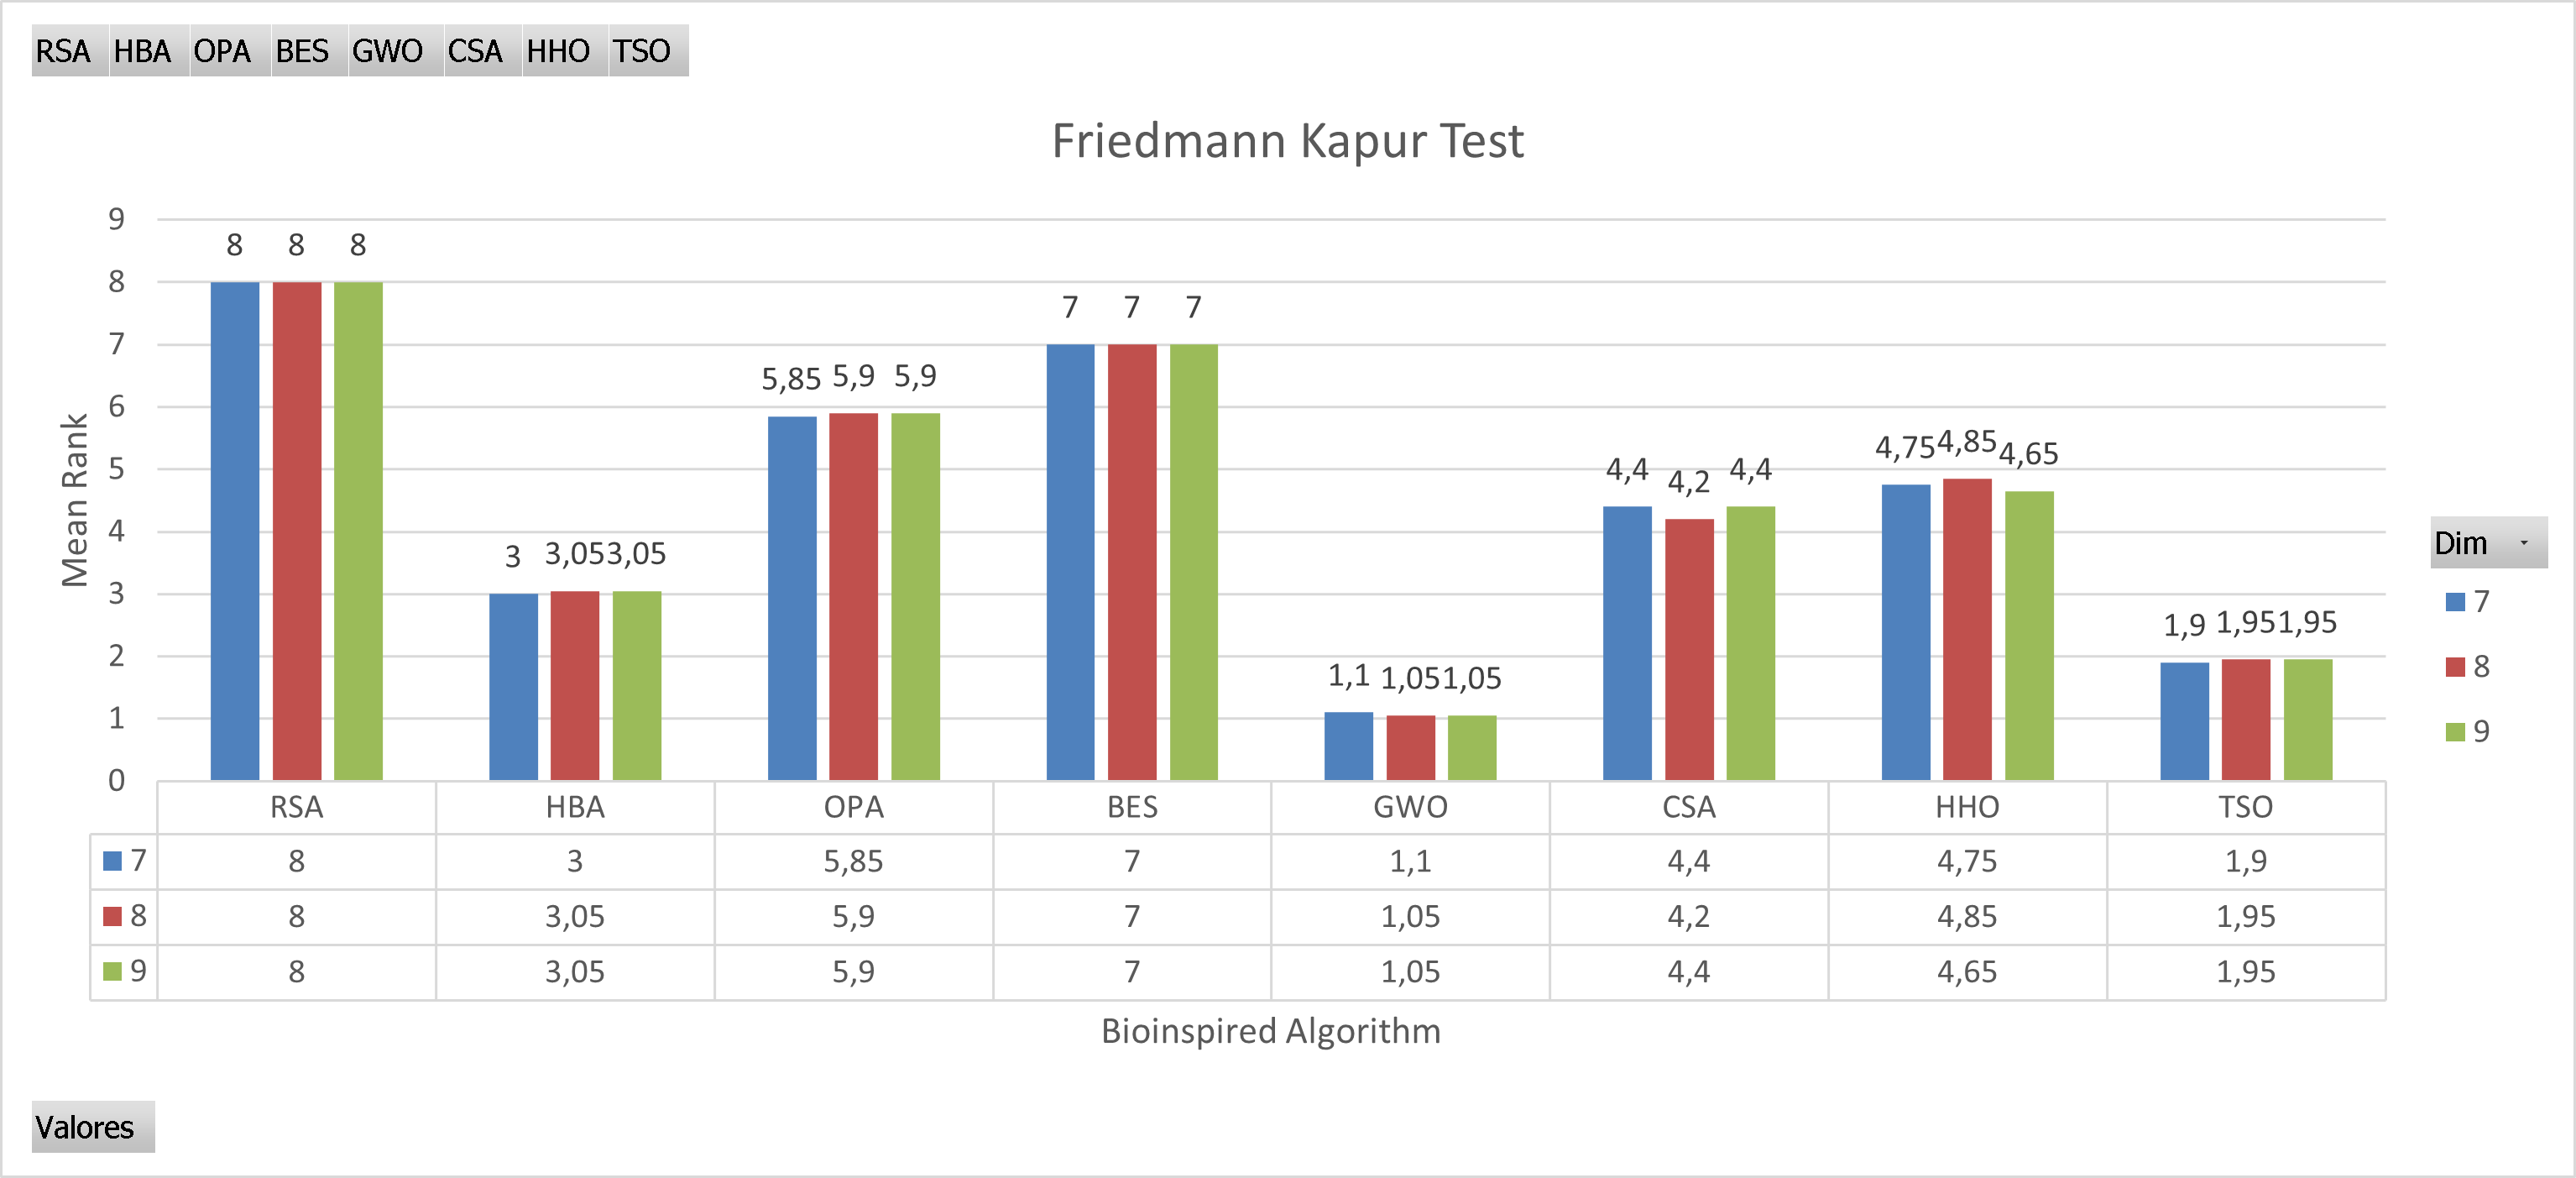
\includegraphics[width=0.8\textwidth]{Fitness/Kapur/Metrica_kapur_Friedman_results.png} \caption{Average fitness metric rank by dimension K and Kapur entropy objective function} \label{fig
} \end{figure}

The analysis of GWO and TSO demonstrated their exceptional effectiveness within the Otsu objective function. TSO achieved impressive average ranks of 1.5, 1.35, and 1.5 in dimensions 7, 8, and 9, respectively, showing consistent high performance across all evaluated dimensions. Similarly, GWO attained top average ranks in the same dimensions, with ranks of 1.5 in dimensions 7 and 9, and 1.65 in dimension 8. Both algorithms showed remarkable adaptability according to the fitness metric and the Otsu objective function, offering robust performance against variations in problem dimensionality.

\begin{figure}[H] \centering 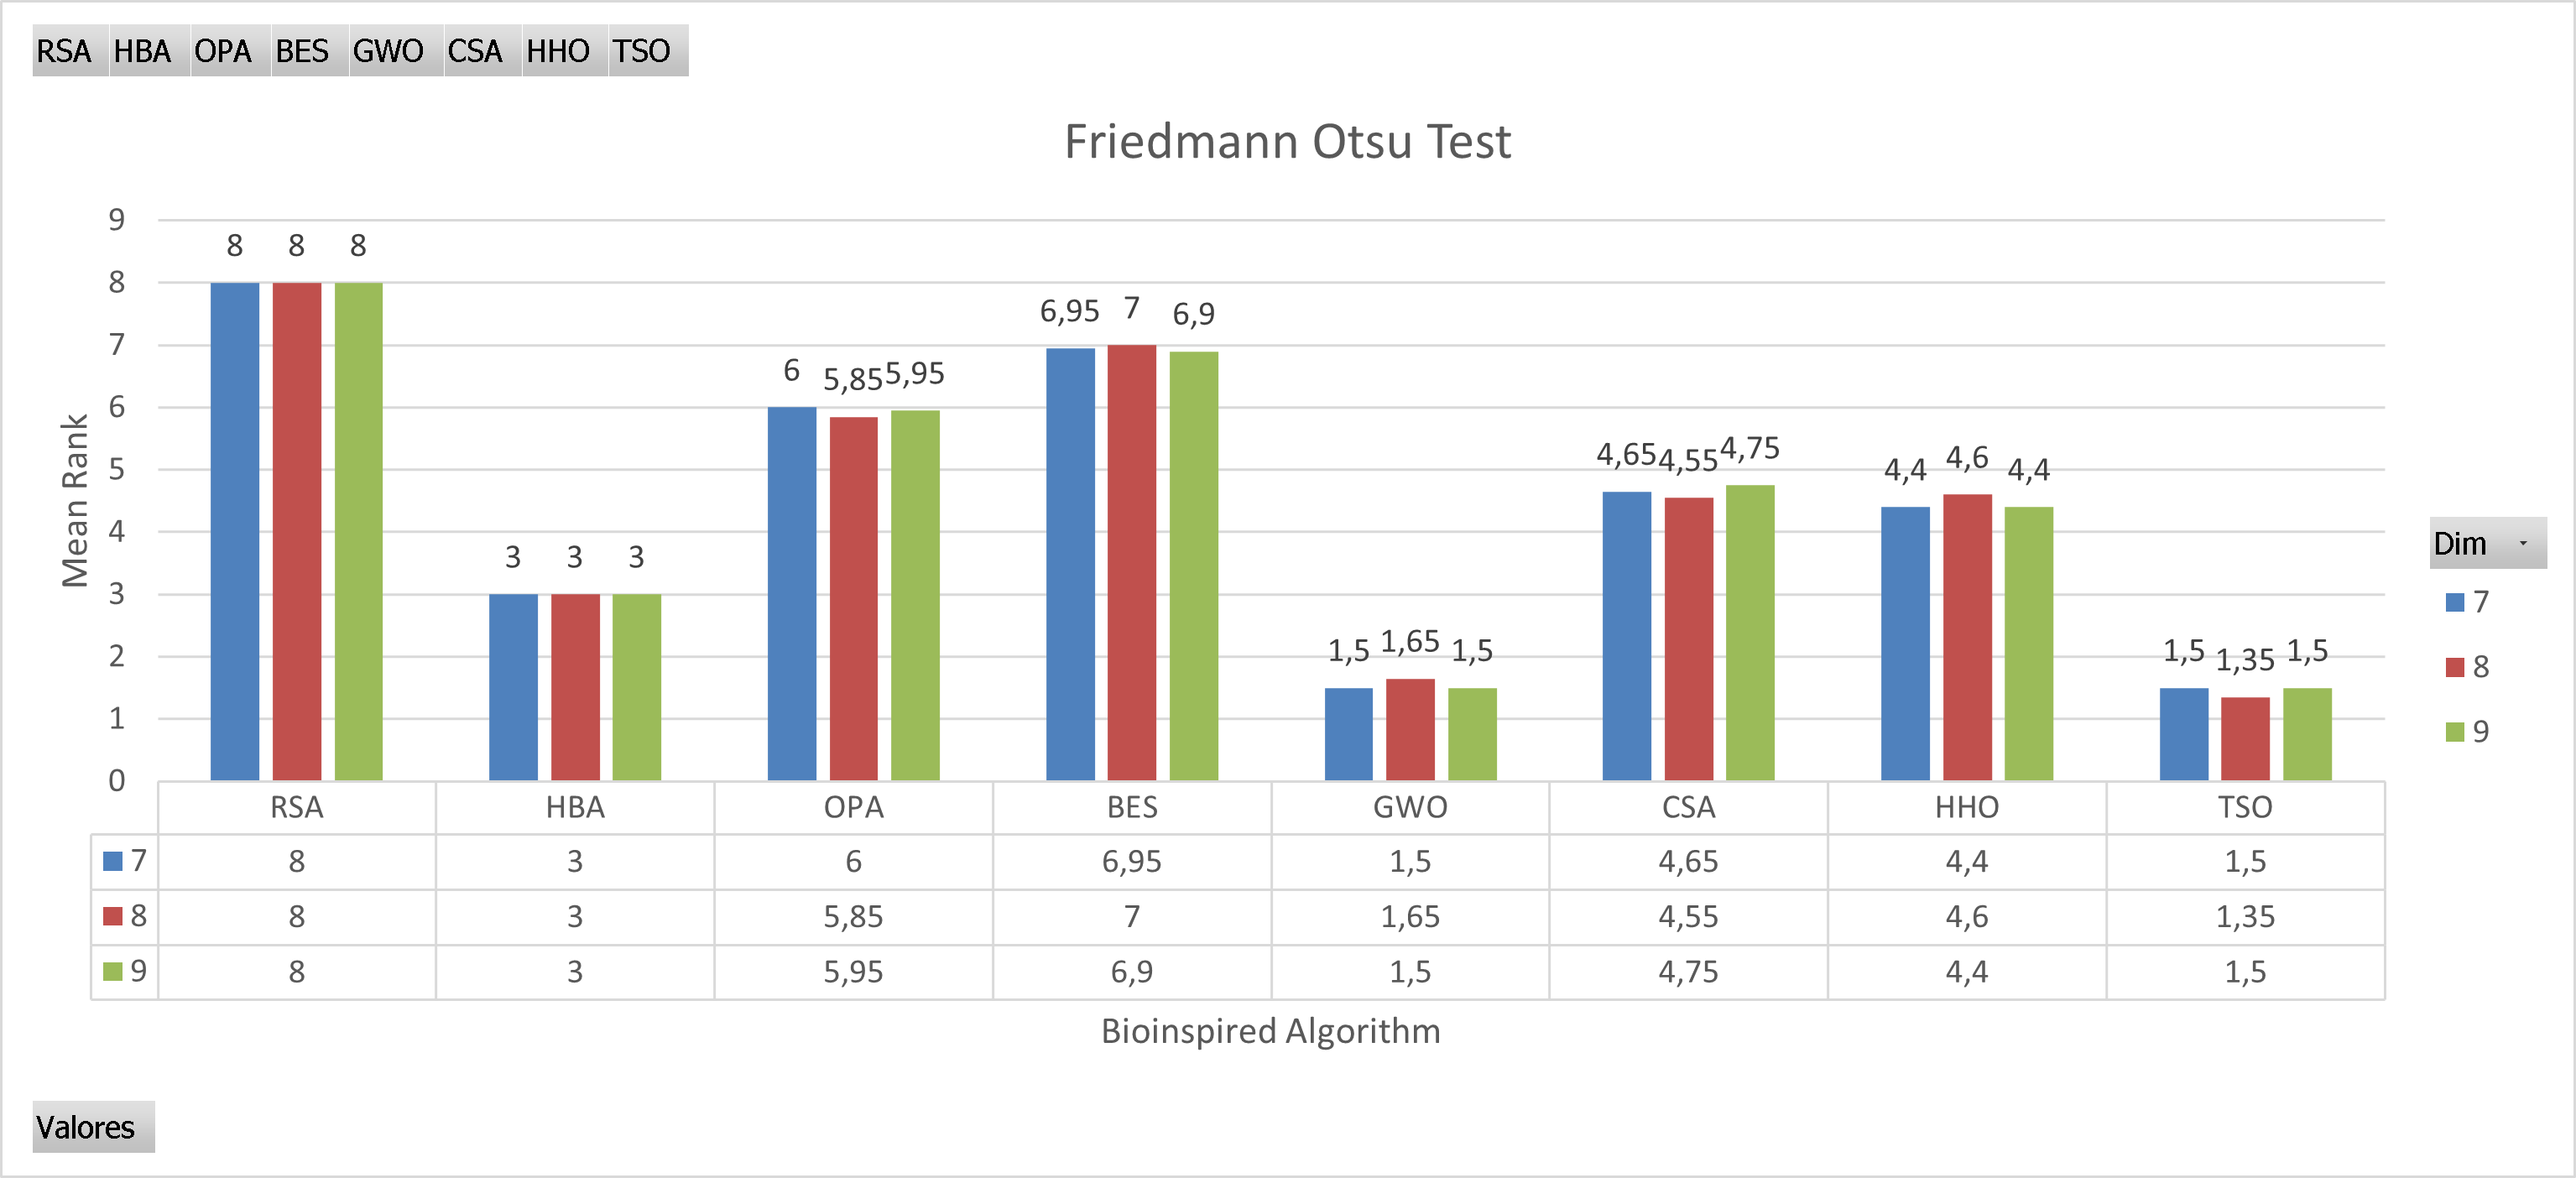
\includegraphics[width=0.8\textwidth]{Fitness/Otsu/Metrica_Otsu_Friedman_results.png} \caption{Average fitness metric rank by dimension K and Otsu objective function} \label{fig
} \end{figure}

The analysis revealed that GWO emerged as the most outstanding performer, achieving the lowest average rank and the best performance with a uniform result of 1.0 across all evaluated dimensions (7, 8, and 9). This consistent excellence underscores GWO’s superiority in the tests conducted. TSO also demonstrated excellent performance, with a constant average rank of 2.0 across all dimensions, positioning it as the second-best algorithm.

\begin{figure}[H] \centering 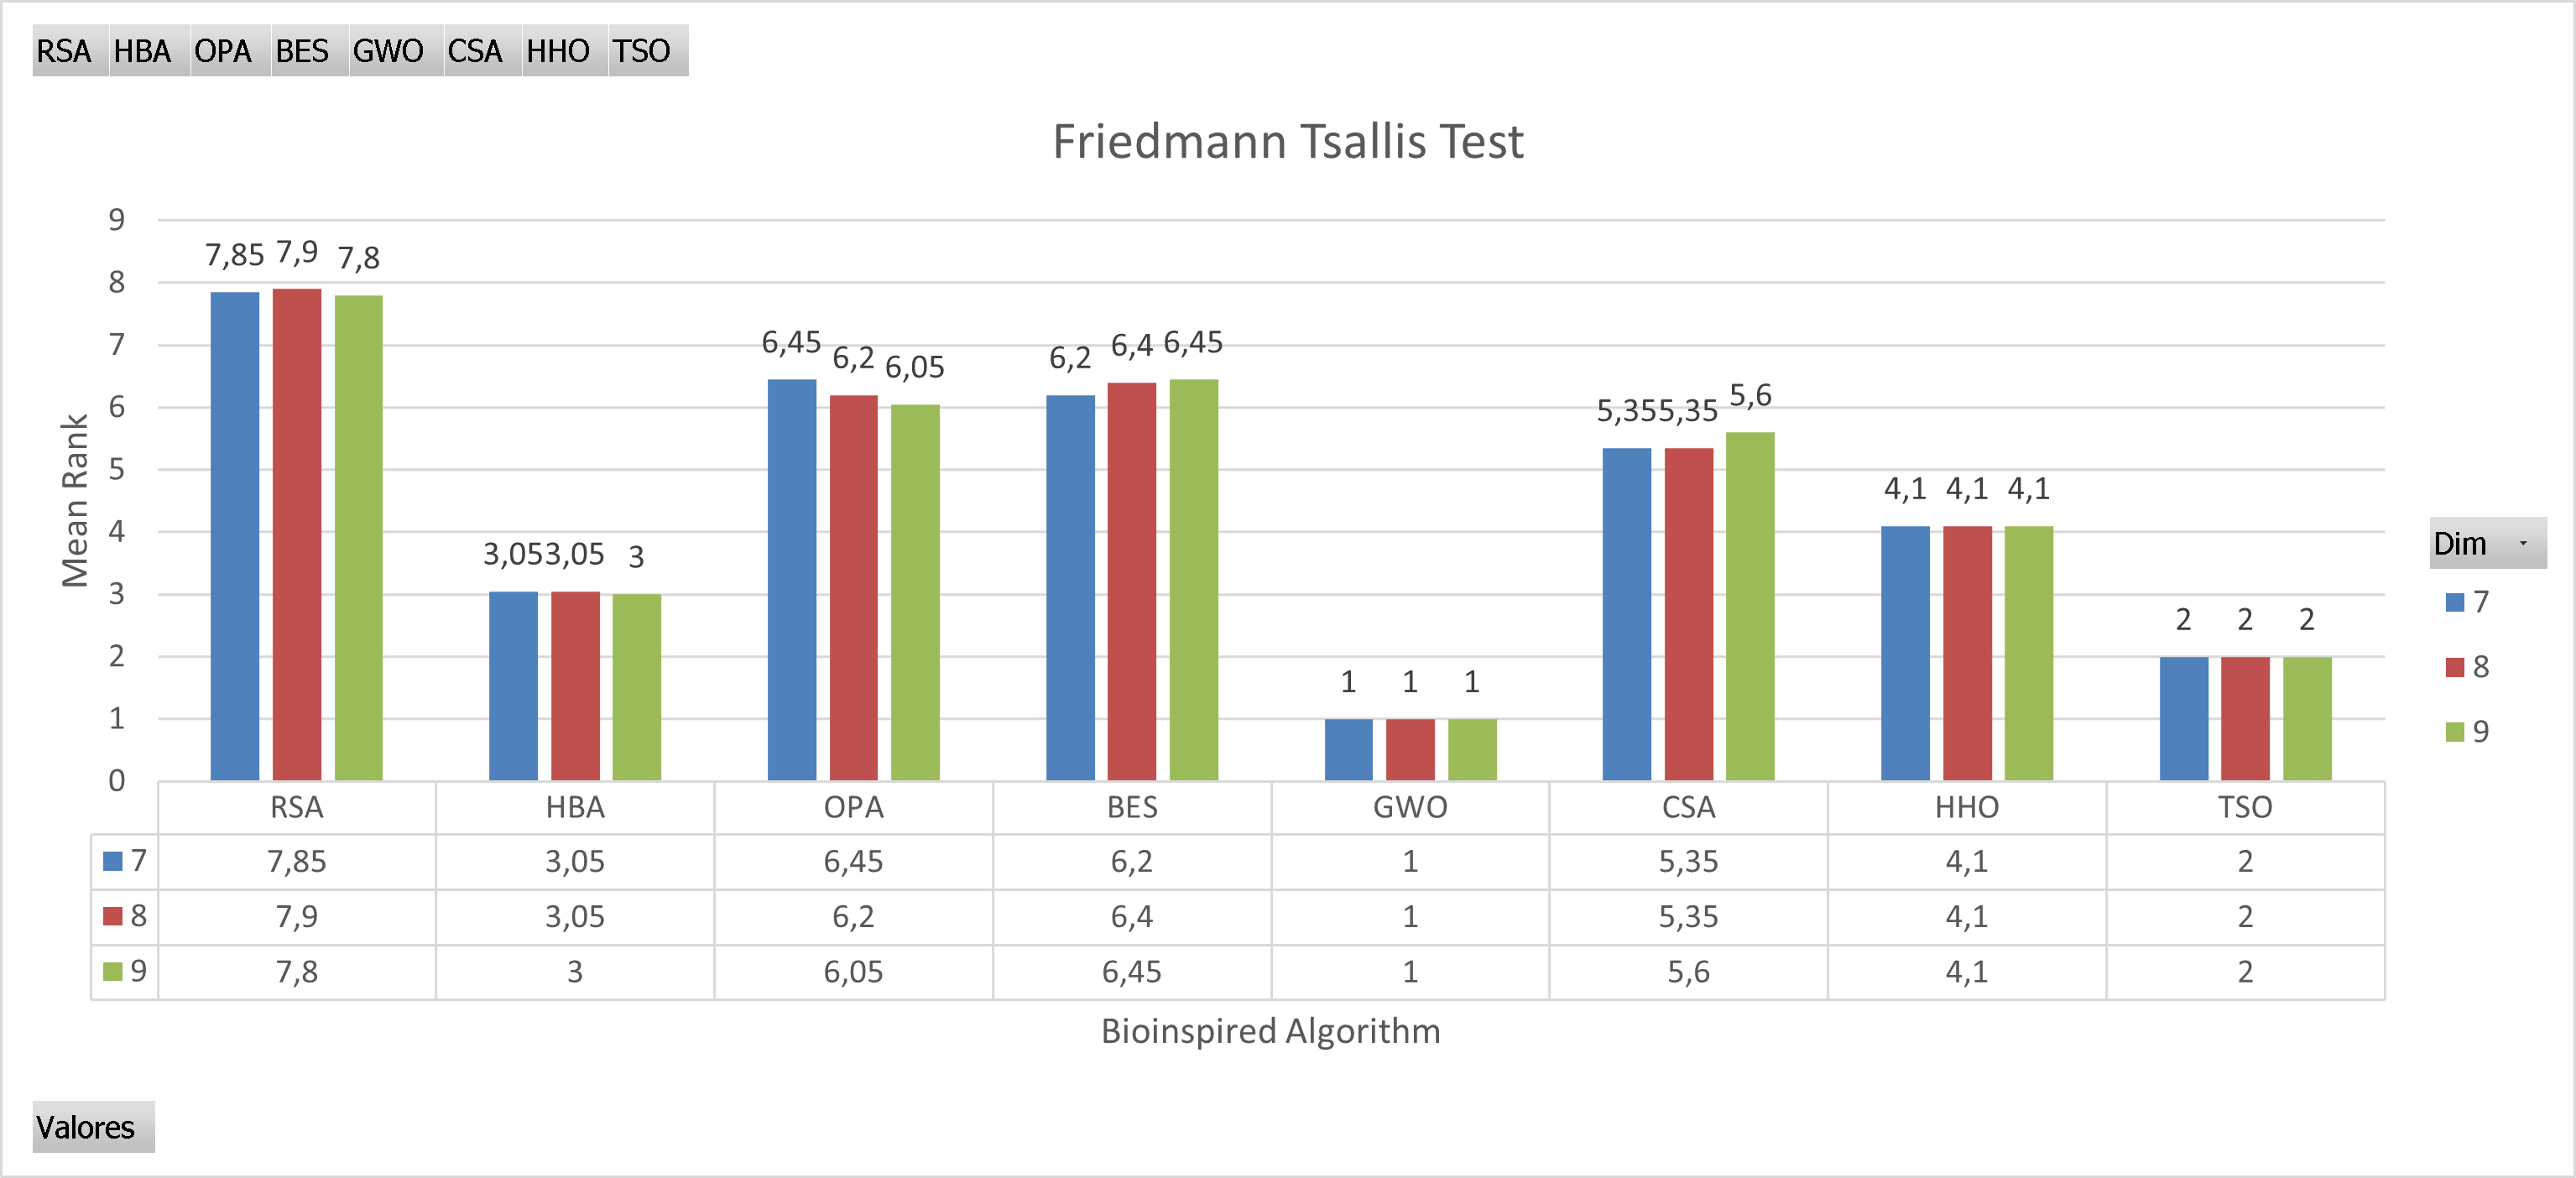
\includegraphics[width=0.8\textwidth]{Fitness/Tsallis/Metrica_Tsallis_Friedman_results.png} \caption{Average fitness metric rank by dimension K and Tsallis objective function} \label{fig
} \end{figure}


\section{Discussion of results} \label{sec:di}

Research on the segmentation of brain images using metaheuristic optimization algorithms has revealed fundamental aspects of the performance of these techniques in a highly specialized medical context. The results provide significant evidence of the efficacy of these algorithms, particularly the Grey Wolf Optimizer GWO, in enhancing the quality and accuracy of magnetic resonance image segmentation.

In Figure \ref{fig:Segmentacion}, four different cases of segmentation in magnetic resonance images are presented, each with an increasing level of structural complexity. This selection illustrates the adaptability and efficiency of the employed segmentation algorithms in the face of various diagnostic challenges.

\begin{figure}[H]
\centering
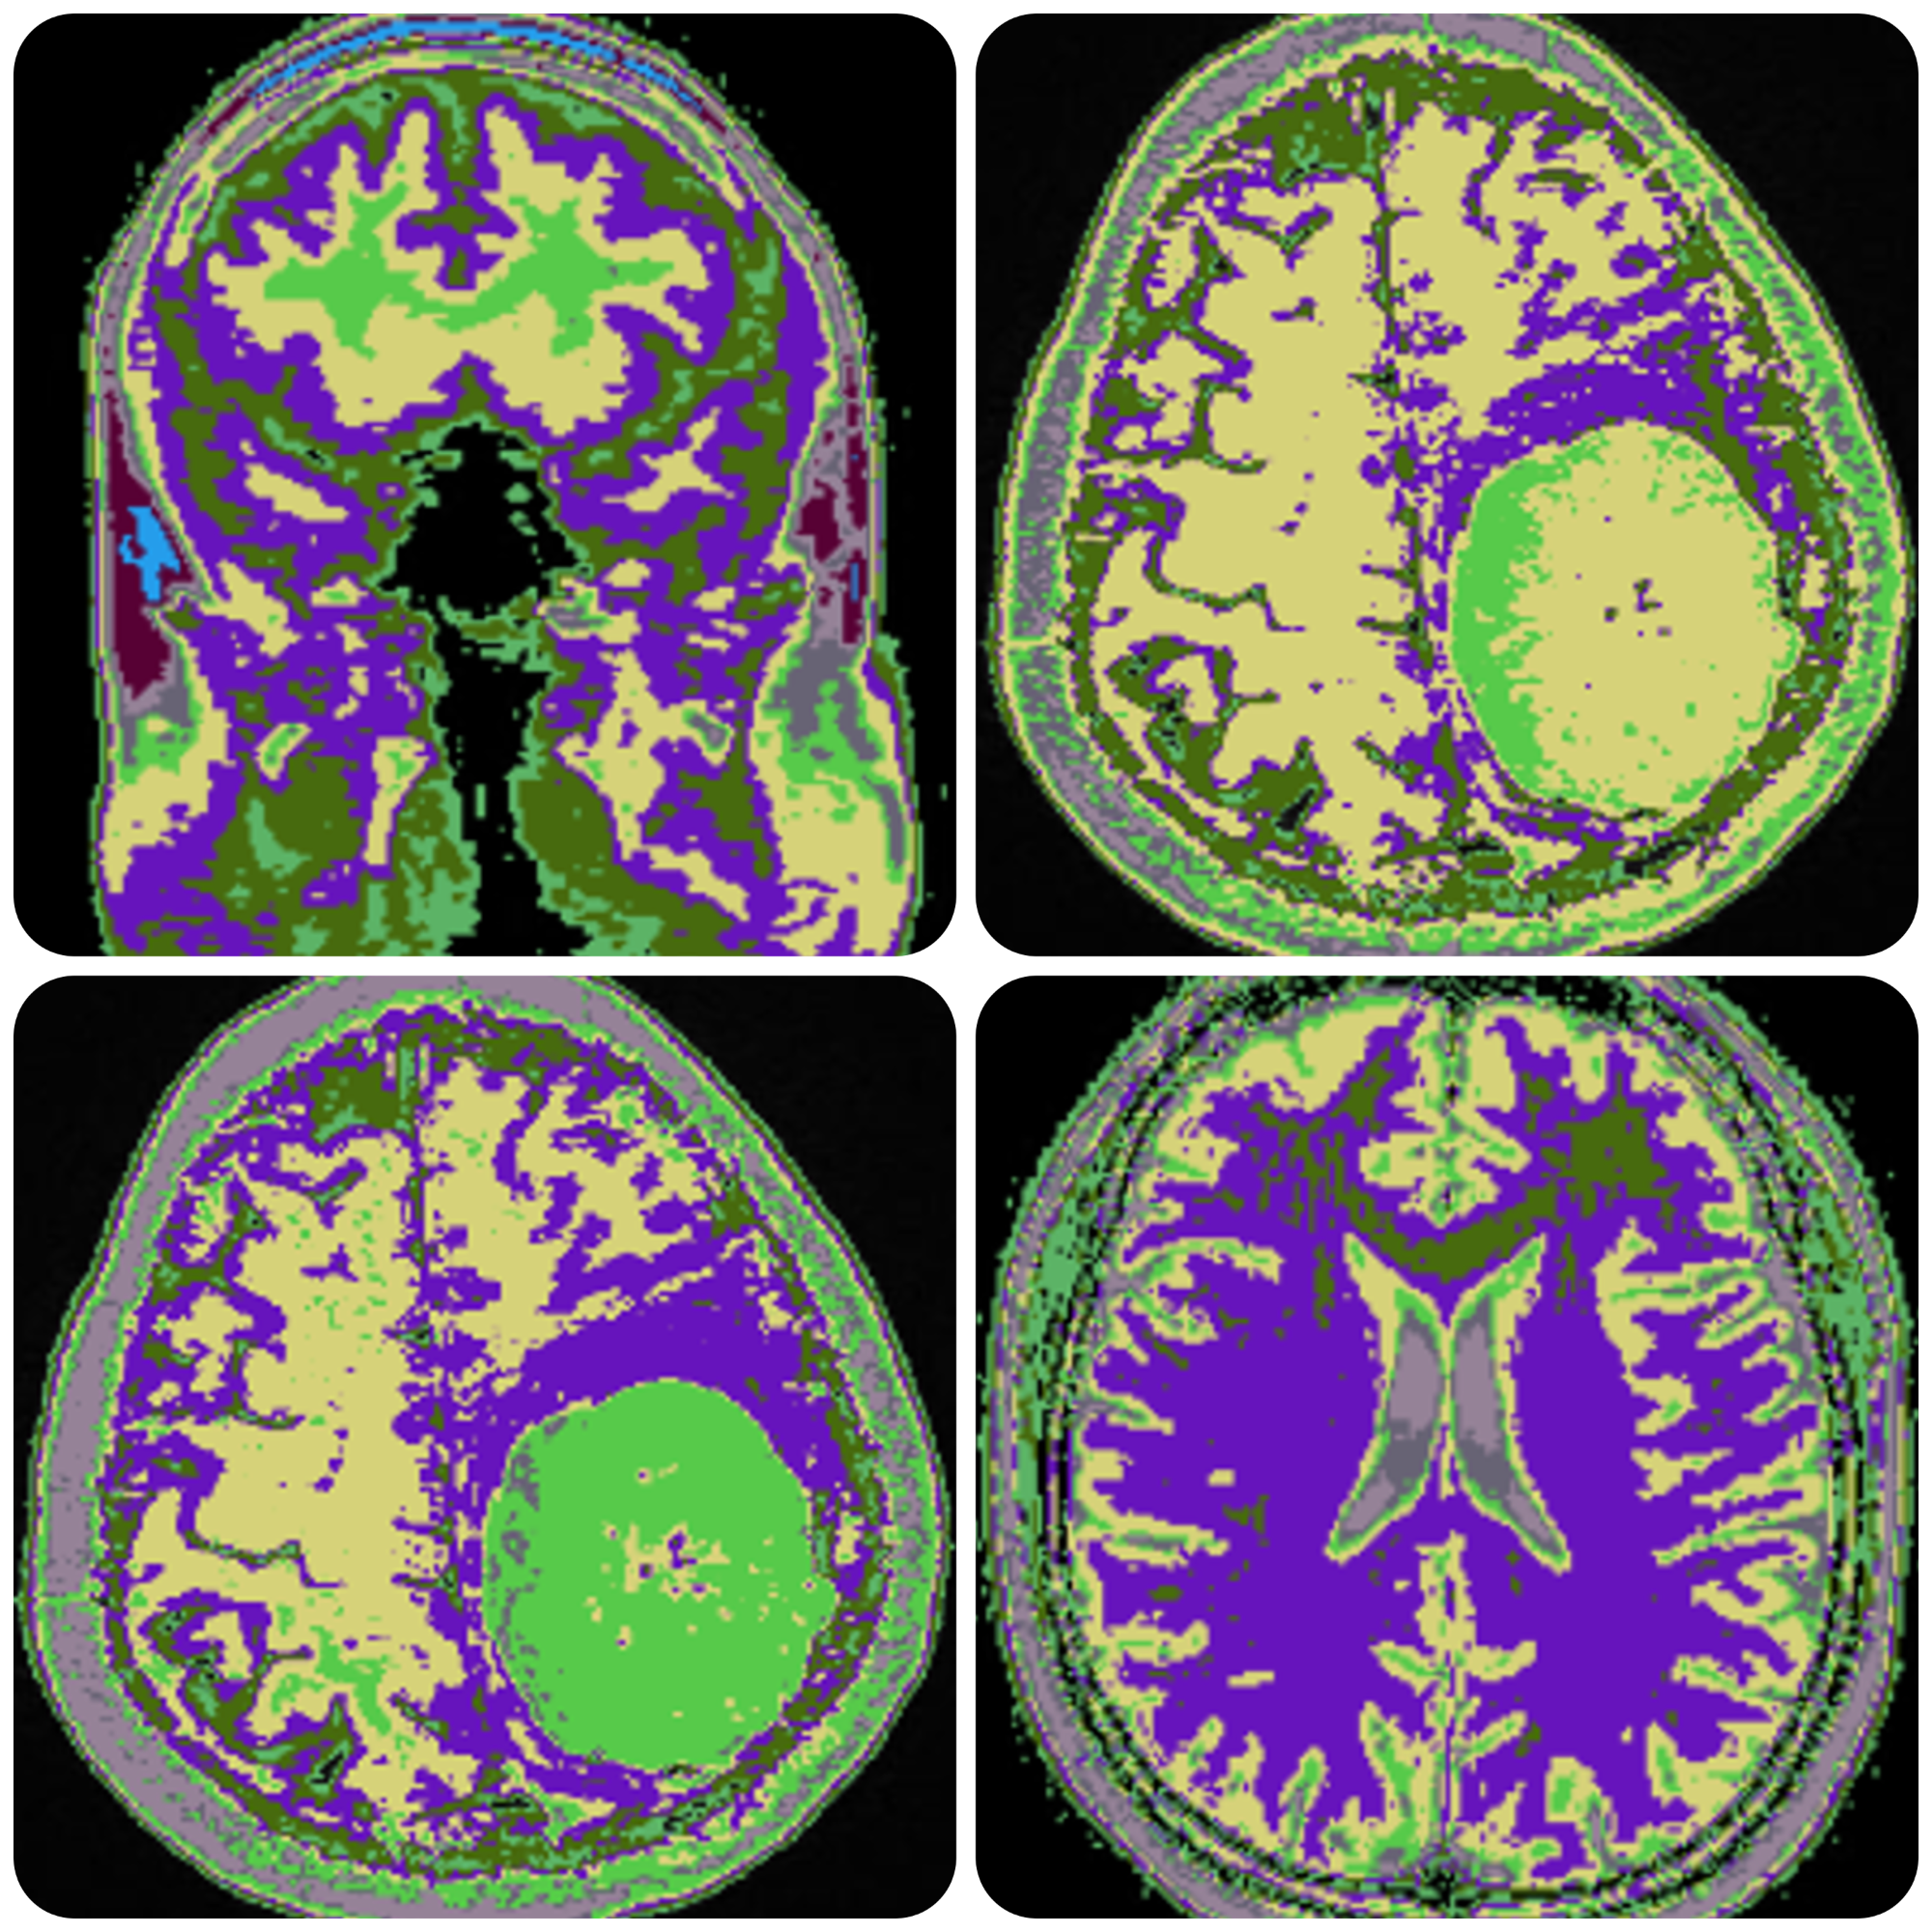
\includegraphics[width=0.5\textwidth]{img/Segmentacion_Discucion.png}
\caption{Comparison of segmentation in medical images with varying levels of structural complexity.}
\label{fig:Segmentacion}
\end{figure}

These results highlight not only the robustness of the segmentation methods used but also their potential to adapt to a wide range of clinical scenarios, making them valuable tools for diagnosis and treatment planning in neurology.

The analysis of the algorithms under different metrics (fitness, PSNR, and SSIM) revealed that although there is variability in performance among the algorithms, some consistently stand out. For example, GWO demonstrated superior performance across almost all metrics and conditions, suggesting its robustness and adaptability to different types of images and segmentation requirements. This consistency is crucial in medical applications, where precision and reliability are of utmost importance for effective diagnosis and treatment.

The fitness function, which measures the quality of segmentation in terms of a predefined goal, was particularly useful for assessing how the algorithms optimize the segmentation process. The results showed that GWO and other algorithms, such as the Honey Badger Algorithm and Tuna Swarm Optimization, were able to effectively explore the search space, finding optimal or near-optimal solutions under various conditions. This exploration capability is essential to adapt to the natural variability present in medical images.

As for the PSNR, which measures the signal-to-noise ratio and hence the preservation of image quality, the results once again highlighted the efficacy of GWO and HBA. These algorithms not only achieved high PSNR values but also showed low variability in their performance, indicating consistent preservation of image quality across different samples. This feature is vital to ensure that segmentation does not degrade the essential information contained in medical images.

The SSIM, which assesses the structural similarity between the segmented image and the original, is another critical metric in medical image segmentation. Algorithms that achieved high SSIM values, such as GWO and HBA, demonstrated their ability to maintain the essential structural characteristics of the images, crucial for medical applications where the accuracy of anatomical structure is paramount.

The influence of dimension K on the performance of the algorithms was also examined. Although general improvements in segmentation quality with an increase in K were observed, no direct and uniform correlation between K and algorithm performance was found. This suggests that the choice of K must be carefully considered and tailored to each specific situation, balancing the need for precision with computational complexity.

The variability in algorithm performance across different images underscores the importance of careful algorithm selection and parameterization for each type of image. This is particularly relevant in a clinical setting, where images can vary significantly in terms of quality, type of tissue represented, and presence of pathologies.

Overall, the results of this study are promising for the application of metaheuristic optimization algorithms in the medical field. The outstanding performance of certain algorithms in the precise segmentation of brain opens new possibilities for the diagnosis and treatment of brain diseases. However, it is crucial to consider the limitations and challenges associated with applying these techniques, such as the need for fine-tuning and detailed evaluation for each specific case.

\section{Conclusion} \label{sec:co}

This research provides important insights into the use and efficacy of metaheuristic optimization algorithms in the segmentation of medical images. The results emphasize the need for careful selection and tuning of these algorithms to fully leverage their capabilities in medical contexts, thereby enhancing the quality of diagnosis and treatment of diseases related to brain parenchyma.

There are significant differences in terms of the fitness metric. The descriptive statistical analysis indicates that the GWO algorithm has the highest mean and the smallest standard deviation, suggesting stability in its results during the 30 executions for all images and their dimensions. Similarly, the TSO algorithm obtained quite similar results but presents a much higher standard deviation than GWO. The Friedman test provides sufficient evidence to determine that the GWO algorithm exhibits a significant difference in performance compared to the rest of the algorithms.

Regarding the PSNR metric, the descriptive statistical analysis does not provide relevant information for analyzing the performance of the algorithms. On the other hand, the Friedman test provides sufficient evidence to determine that the GWO, CSA, HBA, and OPA algorithms showed a significant difference in performance compared to the other algorithms in the PSNR metric for all 20 images and across all dimensions.

The analysis of the results for the SSIM metric using descriptive statistics positions the GWO algorithm as one of the most stable, given its high mean and low standard deviation. Similarly, the Friedman test indicates that GWO is the algorithm that obtained the highest rank value, followed by HBA and OPA, showing a significant difference in performance for the SSIM metric. These results are valid for all images and their dimensions.

Finally, it is concluded that the GWO algorithm exhibits the best overall performance. However, it is necessary to highlight that these results are subject to the nature of the data, the complexity of the images, and the context in which the brain image segmentation is used with the GWO algorithm.

\section*{Acknowledgement}
R. Olivares is supported by grant ANID / FONDECYT / INICIACION / 11231016. F. Ram\'irez and E. Flores are supported by Programa de Doctorado en Ingenier\'ia Informática Aplicada - Universidad de Valpara\'iso.

\bibliographystyle{elsarticle-num}
\bibliography{references}
\end{document}